\section{Diseño y resolución}

En este apartado vamos a pasar a explicar los detalles del desarrollo del proyecto. Como se ha dicho, el proyecto consiste en realizar un sistema capaz de seguir los movimientos del balón y las jugadoras de un partido de volleyball mediante imágenes proporcionadas por una cámara en vista cenital.

El seguimiento se puede realizar por \textit{tracking}, sustracción de fondo, o bien un sistema que aúne ambas cosas para una mayor robustez.

Una vez resuelta la parte del seguimiento, el siguiente objetivo sería registrar las posiciones detectadas a un fichero de salida en formato CSV, mediante el cual se puedan hacer análisis de distintas métricas del juego.

El desarrollo se va a centrar, como he ido aclarando, en una aplicación en Python utilizando OpenCV y PyQt para la parte de interfaz gráfica. De cara a la construcción del sistema, la estrategia a seguir es desarrollar separadamente sus partes y posteriormente implementarlas para que funcionen de manera conjunta.

A continuación, detallaré estas partes y cómo se ha resuelto su implementación. Las partes principales del sistema son: sustracción de fondo, seguimiento (\textit{tracking}), interfaz gráfica y métodos de consistencia temporal.

\subsection{Sustracción de fondo}
Para empezar a detectar formas en la imagen, primero nuestro sistema tiene que ser capaz de hacer una estimación del fondo. La técnica mediante la cual se hace esto se denomina sustracción de fondo. Esta es, por tanto, una parte primordial de nuestro sistema que debe funcionar de una manera suficientemente robusta. Este debe ser capaz, además, de distinguir a las jugadoras del balón, y de etiquetar cada una de las formas de una manera consistente entre los frames del vídeo. Para lograr esta serie de objetivos, no bastará con la salida de los subtractores, sino que tendremos que procesarla con una serie de operaciones.

No obstante, primero tendremos que solucionar el problema principal, la sustracción de fondo. Teniendo en cuenta que las imágenes proceden de una cámara fija y cenital, y que por tanto el fondo siempre va a ser exactamente el mismo, una primera aproximación ingenua a este problema podría ser tan simple como realizar una diferencia entre los frames del video, usando como referencia un frame donde se vea solamente el campo sin ninguna jugadora sobre él.

Por desgracia, las condiciones de iluminación no siempre van a ser totalmente iguales, lo cual va a dificultar en gran medida la detección de objetos usando este método. Además, no siempre vamos a tener disponible una imagen limpia del campo en un vídeo para usar como modelo de fondo. Por ello es complicado realizar un modelo del campo para las diferentes condiciones de iluminación a lo largo de un día mediante resta de frames.

Además de la sensibilidad a cambios en la iluminación, este método adolece de otra desventaja: no es capaz de detectar sombras. Las imágenes que usamos son las de un campo de volleyball dentro de un pabellón, y los focos de dentro de este hacen que sea bastante común tener sombras alargadas y notables en las jugadoras.

Una vez hemos podido ver que esta manera de proceder no es todo lo viable que cabría desear, tendremos que empezar a plantearnos otras opciones a nuestra disposición. OpenCV proporciona distintos algoritmos de sustracción de fondo, los cuales podemos aprovechar y comparar para ver cuál es más apropiado en nuestro propósito.

\begin{figure}
    \centering
    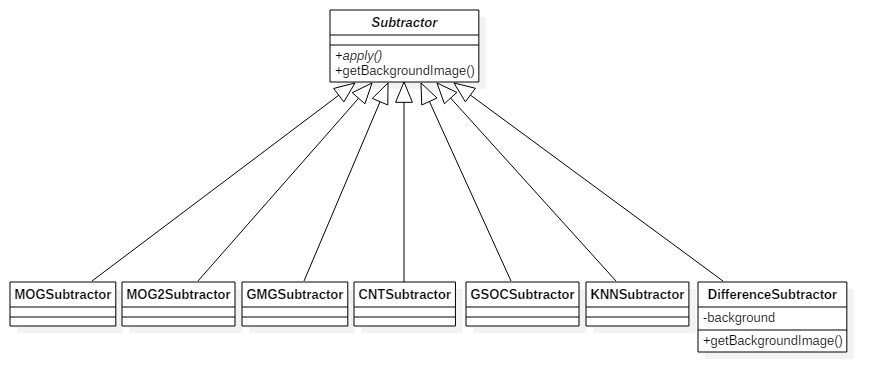
\includegraphics[width=0.9\textwidth]{images/subtractors}
    \caption{Estructura de clases de los sustractores de fondo}
    \label{fig:subtractors}
\end{figure}

Para facilitar el uso de estos algoritmos, se ha hecho uso de la programación orientada a objetos que nos ofrece Python. Se ha creado una clase abstracta llamada Subtractor de la cual heredan todas las clases que hagan uso de los algoritmos de OpenCV así como el de diferencia de frames. Dicha clase proporciona una interfaz común a todas las clases, que hará más sencillo el uso de ellas. La estructura resultante puede verse en la figura \ref{fig:subtractors}.

El funcionamiento interno de las clases resultantes, como se ha dicho, corresponde a las propias implementaciones de OpenCV. Pasaré a explicar los fundamentos teóricos de cada uno de estos algoritmos.

\subsubsection*{MOG}
MOG, mezcla de gaussianas (\textit{Mixture of Gaussians}), fue descrito en  \cite{KaewTraKulPong2002} partiendo de otro algoritmo ya existente de Grimson \textit{et al} \cite{698583,784637,868677}. Usa un modelo de aprendizaje semiparametrizado para estimar el fondo. Ambas versiones crean un modelo del fondo en base a una mezcla de k gaussianas con $3\leq k \leq 5$, cada una de las cuales representa un color. La probabilidad de que un pixel tenga el valor $x_N$ en tiempo N es de
\[
    p(x_N) = \sum_{j=1}^{k} w_j \mathcal{N} (x_N;\theta_j )
\]
donde $w_k$ es el peso de la componente guasiana k-ésima. $\theta(x;\theta_k)$ es la ecuación que define la distribución de la componente, representada por
\[
    \mathcal{N}(x;\theta_k) = \mathcal{N}(x;\mu_k, \Sigma_k) = \frac{1}{(2\pi)^{\frac{D}{2}}|\Sigma_k|^\frac{1}{2}}e^{-\frac{1}{2}(x-\mu_k)^T\Sigma_k^{-1}(x-\mu_k)}
\]
donde $\mu_K$ es la media y $\Sigma_K = \sigma_K^2I$ es la covarianza de la componente. Las distribuciones se ordenan en base a una medida de fitness, definido por $\frac{w_k}{\sigma_k}$ y las B primeras forman el modelo de fondo con $B = \arg\min (\sum_{j=1}^{k} w_j < T)$ donde T es el límite de probabilidad mínima a partir de cual un pixel se considera fondo. Un pixel se considera parte de los objetos de la escena si está 2.5 desviaciones por encima de una de las B distribuciones.

La diferencia entre la implementación original de Grimson y la de este algoritmo es las funciones de actualización de cada frame. En el caso del original las funciones de actualización son: 
\begin{align*}
    &\hat{w}_k^{N+1} = (1 - \alpha)\hat{w}_k^{N} + \alpha\hat{p}(\omega_k | x_{N+1}) \\
    &\hat{\mu}_k^{N+1} = (1 - \alpha)\hat{\mu}_k^{N} + \rho x_{N+1} \\
    &\hat{\Sigma}_k^{N+1} = (1 - \alpha)\hat{\Sigma}_k^{N} + \rho (x_{N+1} - \hat{\mu}_k^{N+1})(x_{N+1} - \hat{\mu}_k^{N+1})^T \\
    &\rho = \alpha \mathcal{N}(x_{N+1};\hat{\mu}_k^N, \hat{\Sigma}_k^N) \\
    &\hat{p}(\omega_k | x_{N+1}) = \text{1 si $\omega_k$ es la primera componente gaussiana; 0 si no}
\end{align*}

Las funciones de actualización de la versión de Kaewtrakulpong añaden ciertas optimizaciones para hacer más robusta la estimación de fondo. Ya que siguen el mismo fundamento que las anteriores, pero son algo más complicadas, no merece la pena explicarlas aquí.

Una novedad de MOG respecto a su predecesor es la capacidad para discernir las sombras de los objetos que las proyectan. El fundamento de ello es emplear una representación cromática de la imagen para reducir la susceptibilidad, aunque también se tiene en cuenta la componente de luminancia. Si un pixel coincide en cromaticidad con la cromaticidad del fondo, y difiere en luminancia por encima de cierto umbral, se marca como sombra.

\begin{figure}
\begin{subfigure}{.5\textwidth}
  \centering
  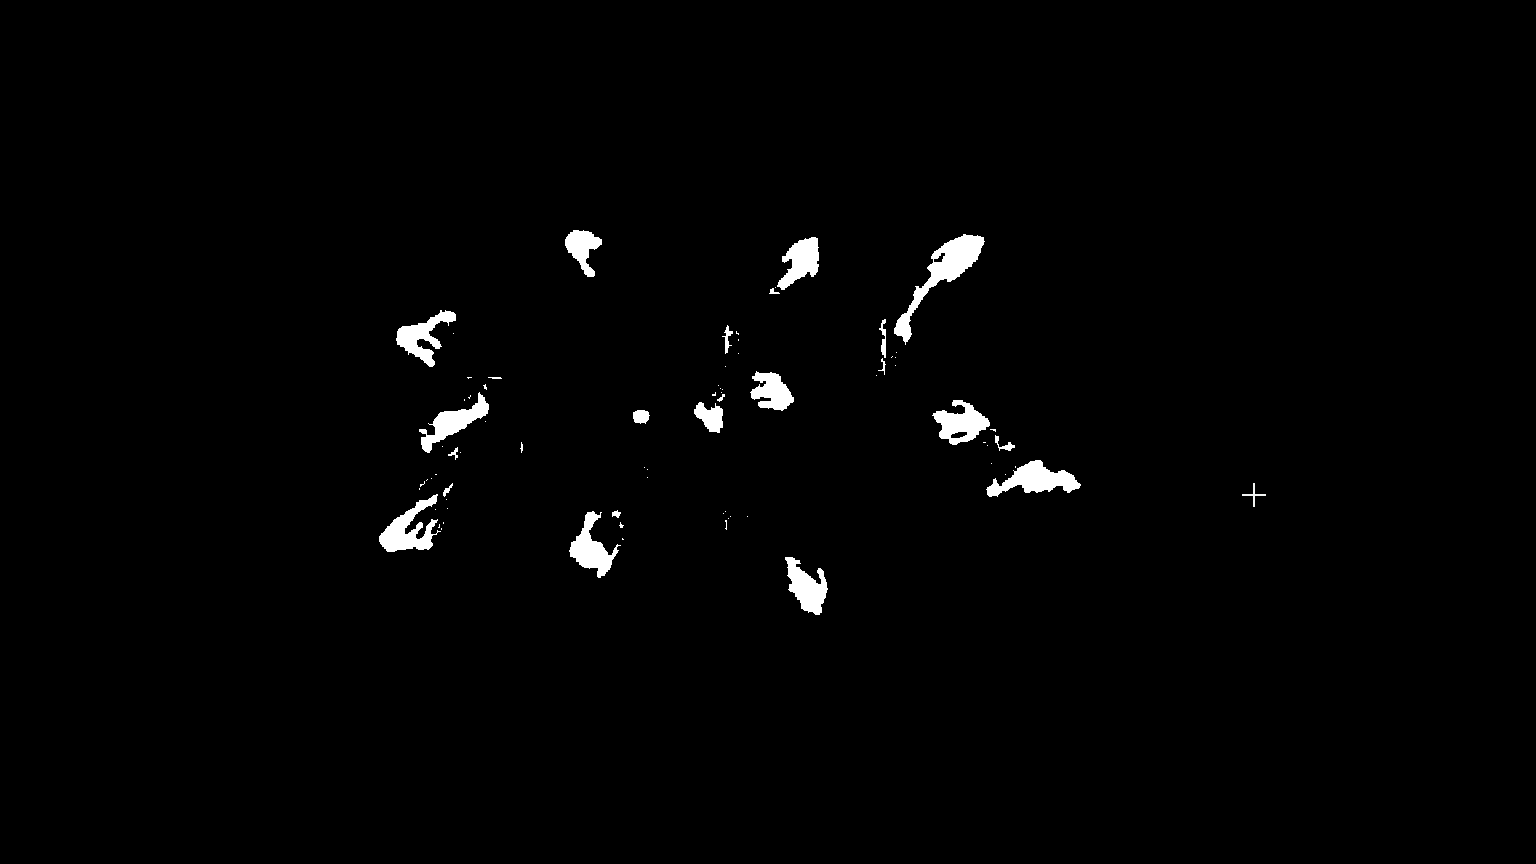
\includegraphics[width=.9\linewidth]{images/MOGsub}
  \caption { }
  \label{fig:MOG1a}
\end{subfigure}%
\begin{subfigure}{.5\textwidth}
  \centering
  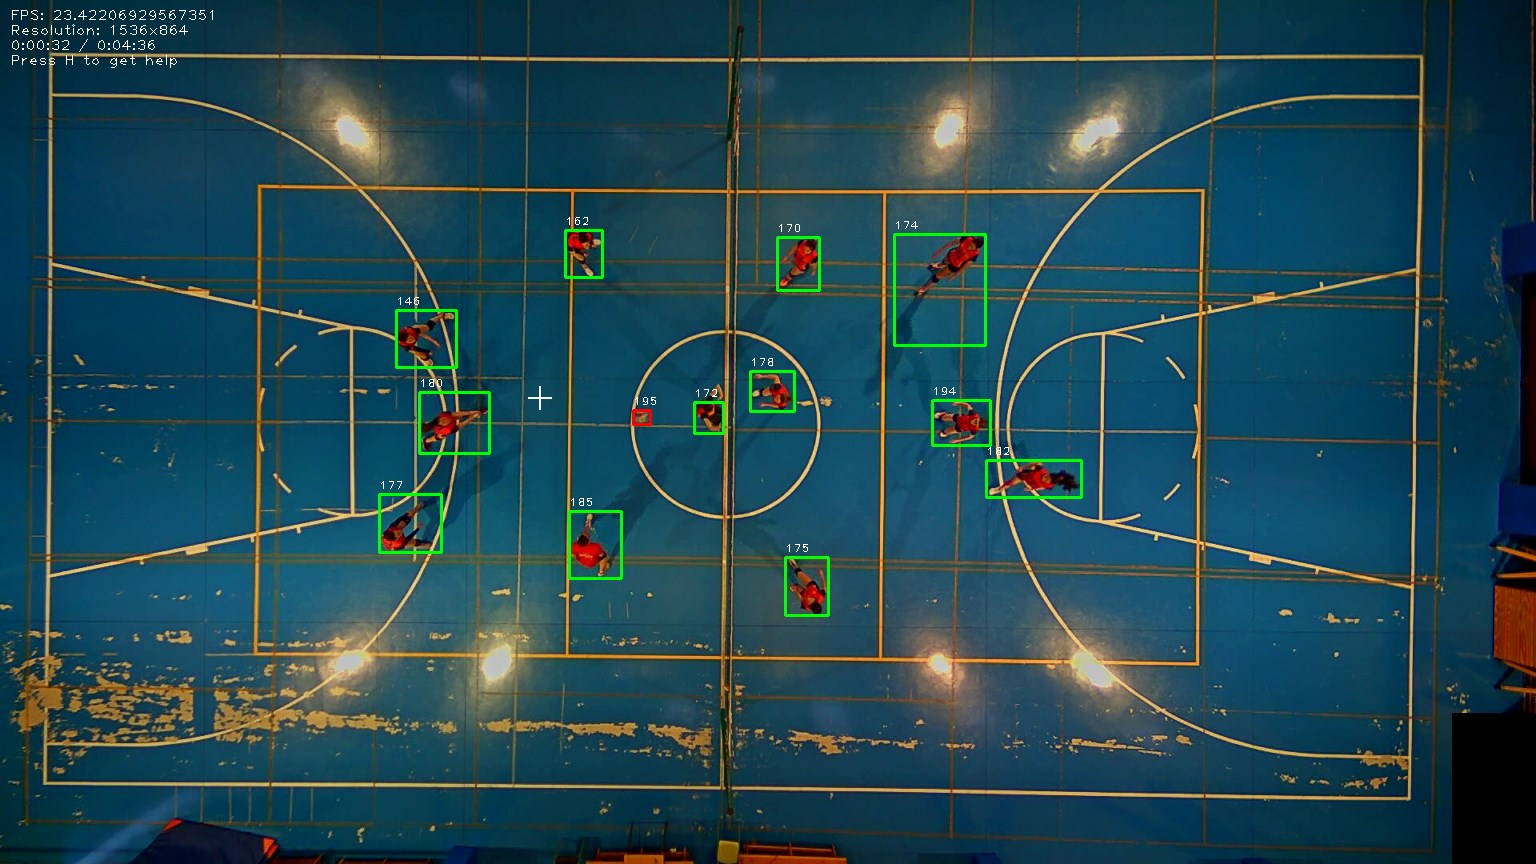
\includegraphics[width=.9\linewidth]{images/MOG}
  \caption { }
  \label{fig:MOG1b}
\end{subfigure}
\caption{Salida del algoritmo MOG (a) Imagen binarizada del algoritmo (b) Imagen del vídeo tras aplicar la máscara}
\label{fig:MOG}
\end{figure}

El funcionamiento de MOG en un frame puede verse en la figura \ref{fig:MOG}, como puede verse, el algoritmo detecta los cuerpos con cierto nivel de fidelidad, aunque en algunos momentos puede ser especialmente sensible a una jugadora estática. Por otro lado, la detección de las sombras no es en absoluto perfecta, y no en pocas ocasiones se marcan partes de la sombra como componentes de la imagen. El rendimiento es correcto, no se aprecian ralentizaciones graves.

\subsubsection*{MOG2}
MOG2 es un algoritmo propuesto en los trabajos \cite{art:Zivkovic1} y \cite{art:Zivkovic2} de Z. Zivkovic. Tiene el mismo fundamento que el anterior método, estima el fondo mediante K gaussianas, haciendo uso nuevamente de un modelo semiparametrizado. 

La diferencia respecto a MOG es que, en lugar de mantener la distrubición de mezcla de K gaussianas para todos los pixeles de la imagen, este método es capaz de adaptarse automáticamente y seleccionar el número de componentes gaussianas necesario para cada pixel. Esto permite una mayor flexibilidad e incluso mayor eficiencia, ya que en el mejor de los casos podría tener pixeles con el mismo número de componentes que usaría el anterior, pero otros con menos, agilizando la computación.

\begin{figure}
\begin{subfigure}{.5\textwidth}
  \centering
  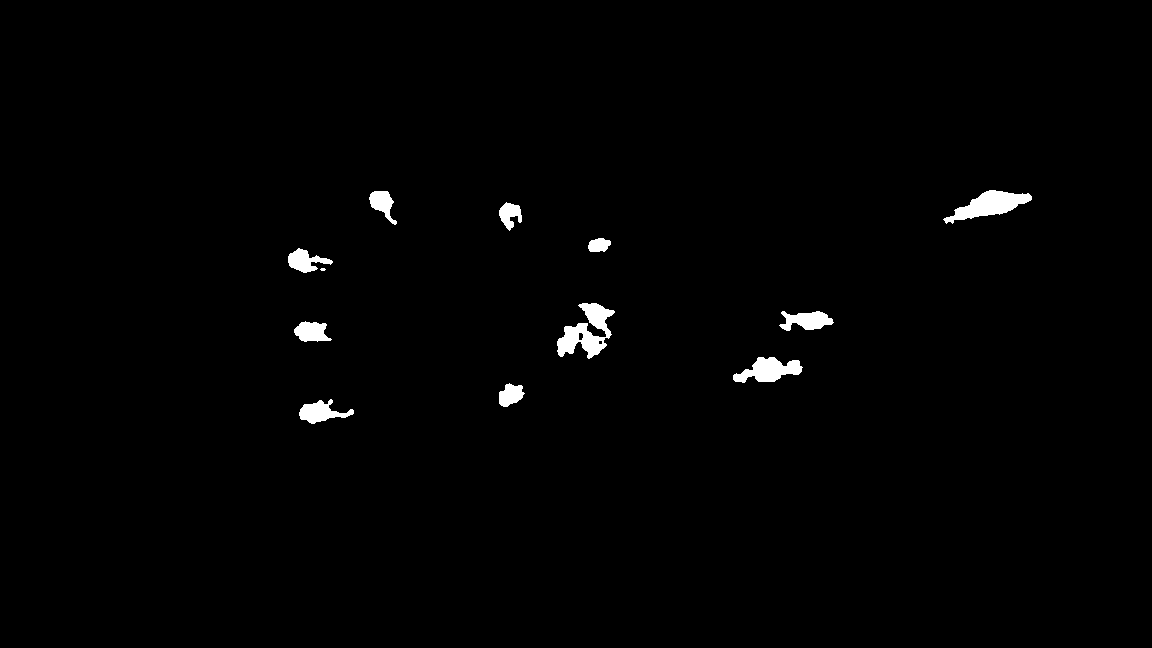
\includegraphics[width=.9\linewidth]{images/MOG2sub}
  \caption { }
  \label{fig:MOG21a}
\end{subfigure}%
\begin{subfigure}{.5\textwidth}
  \centering
  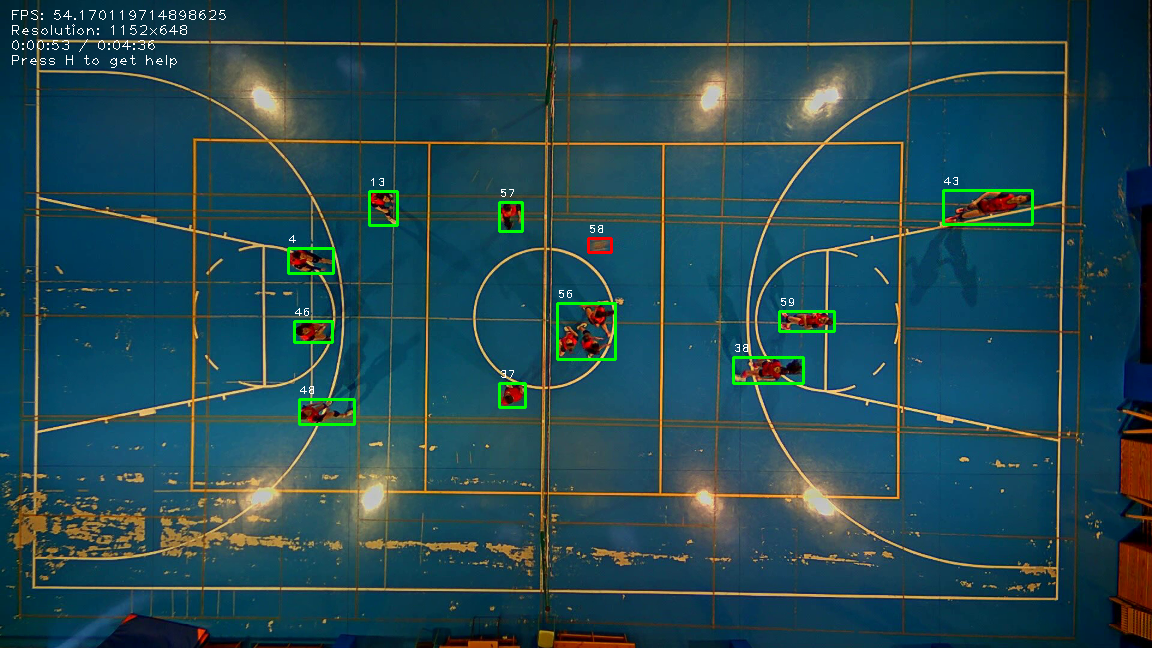
\includegraphics[width=.9\linewidth]{images/MOG2}
  \caption { }
  \label{fig:MOG21b}
\end{subfigure}
\caption{Salida del algoritmo MOG2 (a) Imagen binarizada del algoritmo (b) Imagen del vídeo tras aplicar la máscara }
\label{fig:MOG2}
\end{figure}

\subsubsection*{GMG}
GMG surge en un trabajo de Godbehere \textit{et al.} \cite{art:Godbehere}. En este trabajo aclaran los autores que se inspiraron en los algoritmos ya existentes en OpenCV. A diferencia de MOG y MOG2, que emplean modelos de distribuciones gaussianas para estimar el fondo de la imagen, GMG emplea un histograma. Por tanto, es un modelo no paramétrico.

El método tiene una peculiaridad respecto al resto, y es que requiere de un número $T$ de frames determinado para inicializar el modelo de fondo. Esta inicialización puede ser interesante en caso de contar con vídeos en los que se vea el fondo al principio sin ningún tipo de oclusión, en nuestro caso, que se vea el campo sin ningún jugador. Desgraciadamente, esto no siempre es posible, por lo que la efectividad inicial puede verse limitada debido a esta condición.

Durante la inicialización, se guarda un histograma $\hat{H}_{ij}(k)$ en espacio RGB por cada pixel previamente cuantizado. Los primeros $T$ frames del vídeo se utilizan como datos de entrenamiento para estimar la función de probabilidad de cada pixel, es decir, el modelo de fondo. El proceso de inicialización comienza en cada frame generando un vector $f_{ij}(k) = L(\hat{I}_{ij}(k)) \in \mathcal{F}$ mediante una función $L$ a partir de la entrada. Una vez generados todos los vectores, se calcula el histograma $\hat{H}_{ij}(T) = \frac{1}{F_{tot}}\Sigma_{x = 1}^T f_{ij}(x)$. $F_{tot}$ es el número total de distintas características (\textit{features}) observadas, que siempre debe ser menor o igual que $F_{max}$, una constante del sistema. En caso de que sea mayor, se eliminan las observaciones más antiguas hasta que se cumpla que $F_{tot} \leq F_{max}$.

A partir de aquí se utiliza inferencia bayesiana para calcular la probabilidad de que un pixel dado sea fondo a partir de la característica observada. Sea $p(F|f)$ la probabilidad de que un pixel con característica $f_{ij}(k)$ sea parte del primer plano y $p(B|f)$ la probabilidad de que este mismo pixel sea fondo:
\[
    p(B|f) = \frac{p(f|B)p(B)}{p(f|B)p(B)+p(f|F)p(F)}
\]

Siendo $p(f|B) = f_{ij}(k)^T\hat{H}_{ij}(k)$, $p(f|F) = 1 - p(f|B)$, $p(F)$ un parámetro constante que afecta a la sensibilidad del algoritmo y $p(B) = 1 - p(F)$. Una vez calculado $p(B|f)$ para cada pixel, obtenemos una imagen $P(k)$ a la que se le aplican una serie de transformaciones morfológicas de manera que se eliminen las posibles pequeñas formas anómalas que puedan detectarse y las componentes de la imagen aparezcan conectadas. Posteriormente, se aplica un umbral a la imagen para generar a partir de ella una imagen en binario que servirá como máscara y será la salida del sustractor.

Por último, se debe actualizar el histograma que se usa como modelo de fondo de manera que se adapte a posibles cambios en la escena. Si un pixel está marcado como frente de la escena, el histograma para él no se actualiza. Si no, si la característica $f_{ij}(k)$ tiene peso 0 en el histograma y se ha excedido la constante $F_max$, se debe eliminar algúna característica del histograma, la de menor peso. A continuación se actualiza el histograma con la nuevo característica a añadir: $H_{ij}(k+1)=(1-\alpha)H_{ij}(k)+\alpha f_{ij}(k)$ siendo $\alpha$ el parámetro de adaptación (\textit{learning rate}) del algoritmo, y cuanto más grande sea, antes se eliminan las observaciones anteriores.

\begin{figure}
\begin{subfigure}{.5\textwidth}
  \centering
  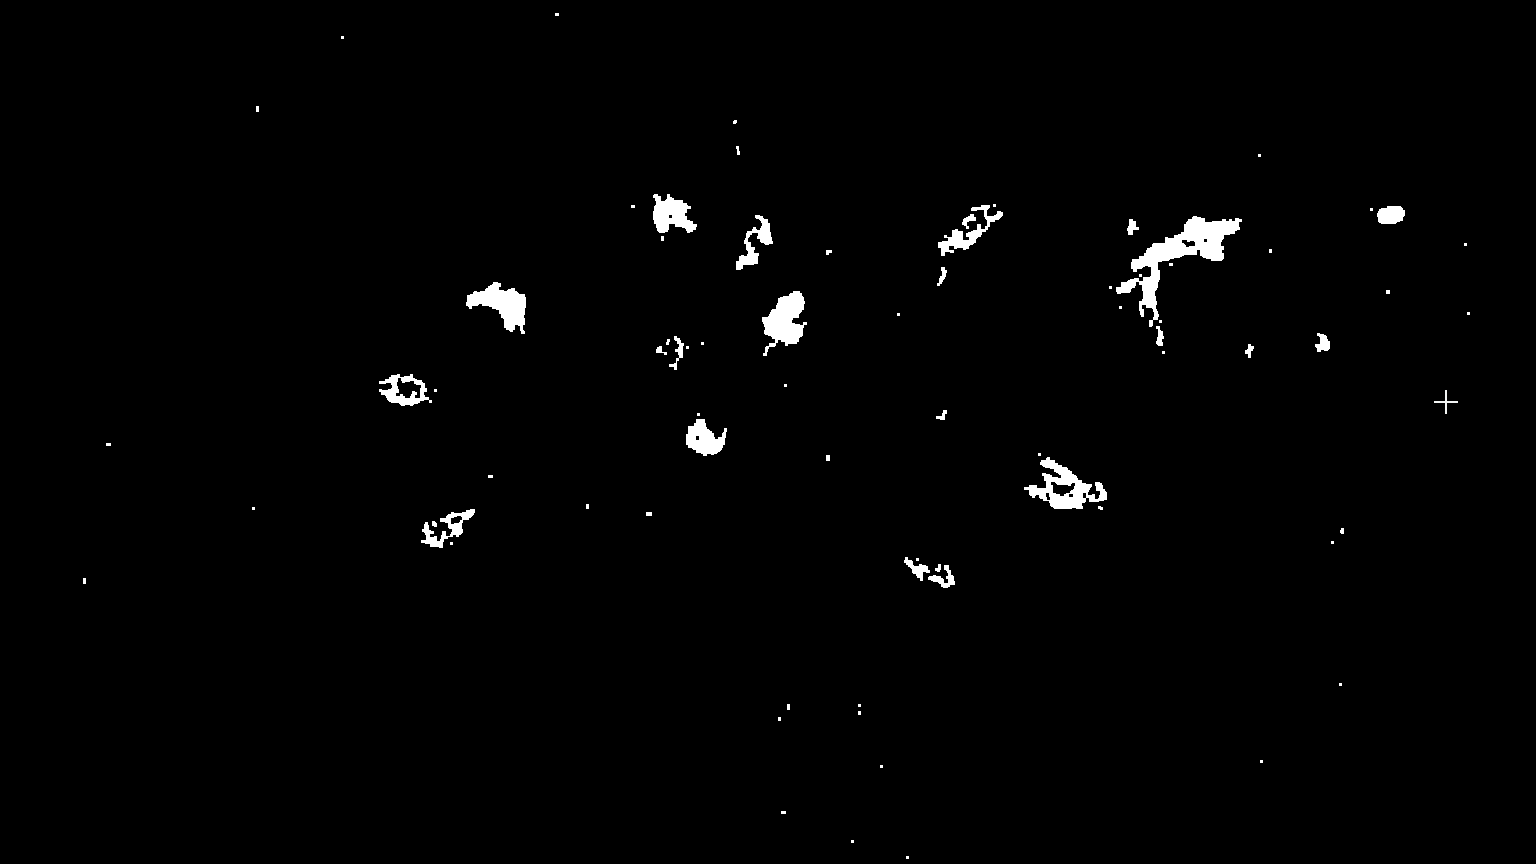
\includegraphics[width=.9\linewidth]{images/GMGsub}
  \caption { }
  \label{fig:GMG1a}
\end{subfigure}%
\begin{subfigure}{.5\textwidth}
  \centering
  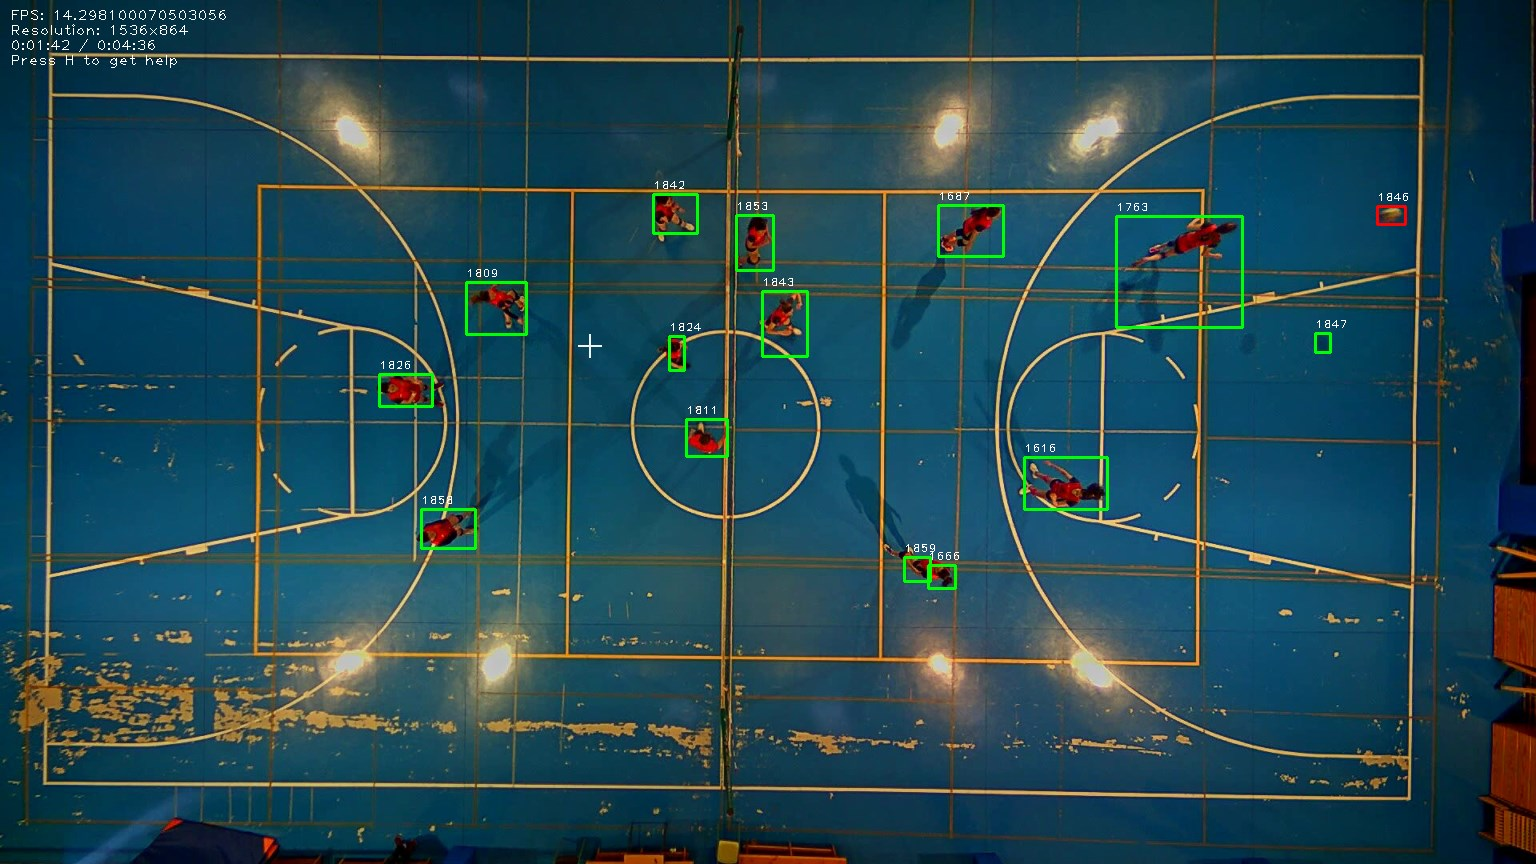
\includegraphics[width=.9\linewidth]{images/GMG}
  \caption { }
  \label{fig:GMG1b}
\end{subfigure}
\caption{Salida del algoritmo GMG (a) Imagen binarizada del algoritmo (b) Imagen del vídeo tras aplicar la máscara }
\label{fig:GMG}
\end{figure}

En cuanto al desempeño del algoritmo, en la figura \ref{fig:GMG} podemos ver que es extremadamente sensible al ruido de la cámara, cosa que hace que la detección de objetos no sea estable. Esta inestabilidad hace que constantemente se pierdan de un frame a otro algunos de los contornos, y haya que asignarles etiquetas nuevas, lo que explica que en la imagen haya etiquetas tan altas. Se aprecian algunos fallos en la detección de sombras, por ejemplo, los de la jugadora más arriba a la derecha y el balón en la imagen. 

El rendimiento no es especialmente bueno, se puede apreciar que cuando el ruido de imagen es muy grande y se detectan muchos contornos falsos, el funcionamiento es extremadamente lento. Además, durante los frames de inicialización, también se notan algunos bajones de FPS. Con todo, estos problemas no son especialmente serios y un reescalado de la imagen bastaría para paliarlos.


\subsubsection*{CNT}
Este método fue desarrollado como open source en \cite{git:CNT}. El algoritmo fue planteado por el desarrollador para que fuera eficiente en máquinas de bajo rendimiento, como raspberryPi. Se basa en ``contar'' (que es de donde viene su nombre) cuántos frames se mantiene estable un pixel, y a mayor estabilidad, mayor probabilidad de que este sea fondo.

El método consta de 2 parámetros principales: minPixelStability y maxPixelStability. La utilidad de estos parámetros es, respectivamente, indicar el número de frames que un pixel debe mantenerse en el mismo color para ser considerado estable, y el máximo crédito que se le permite a un pixel en el histograma.

El algoritmo es relativamente sencillo en su funcionamiento: en cada frame se calcula la diferencia entre el color actual y el del frame anterior, si no se diferencian por encima de cierto límite, se incrementa la estabilidad del pixel en cuestión. Cuando la estabilidad de un pixel llega a ser igual o mayor que la que se le pasa al algoritmo por parámetro se empieza a considerar parte del fondo.

Existe la opción de añadir el uso de un histograma, y aquí es donde cobra importancia el segundo parámetro. Además de llevar un conteo de la estabilidad del propio pixel, se mantiene un histograma con las estabilidades que ha tomado este, y si un pixel supera el valor máximo se deja de sumar. De esta manera el algoritmo puede reponerse rápidamente a que un objeto que ha pasado largo tiempo en escena se mueva.

\begin{figure}
\begin{subfigure}{.5\textwidth}
  \centering
  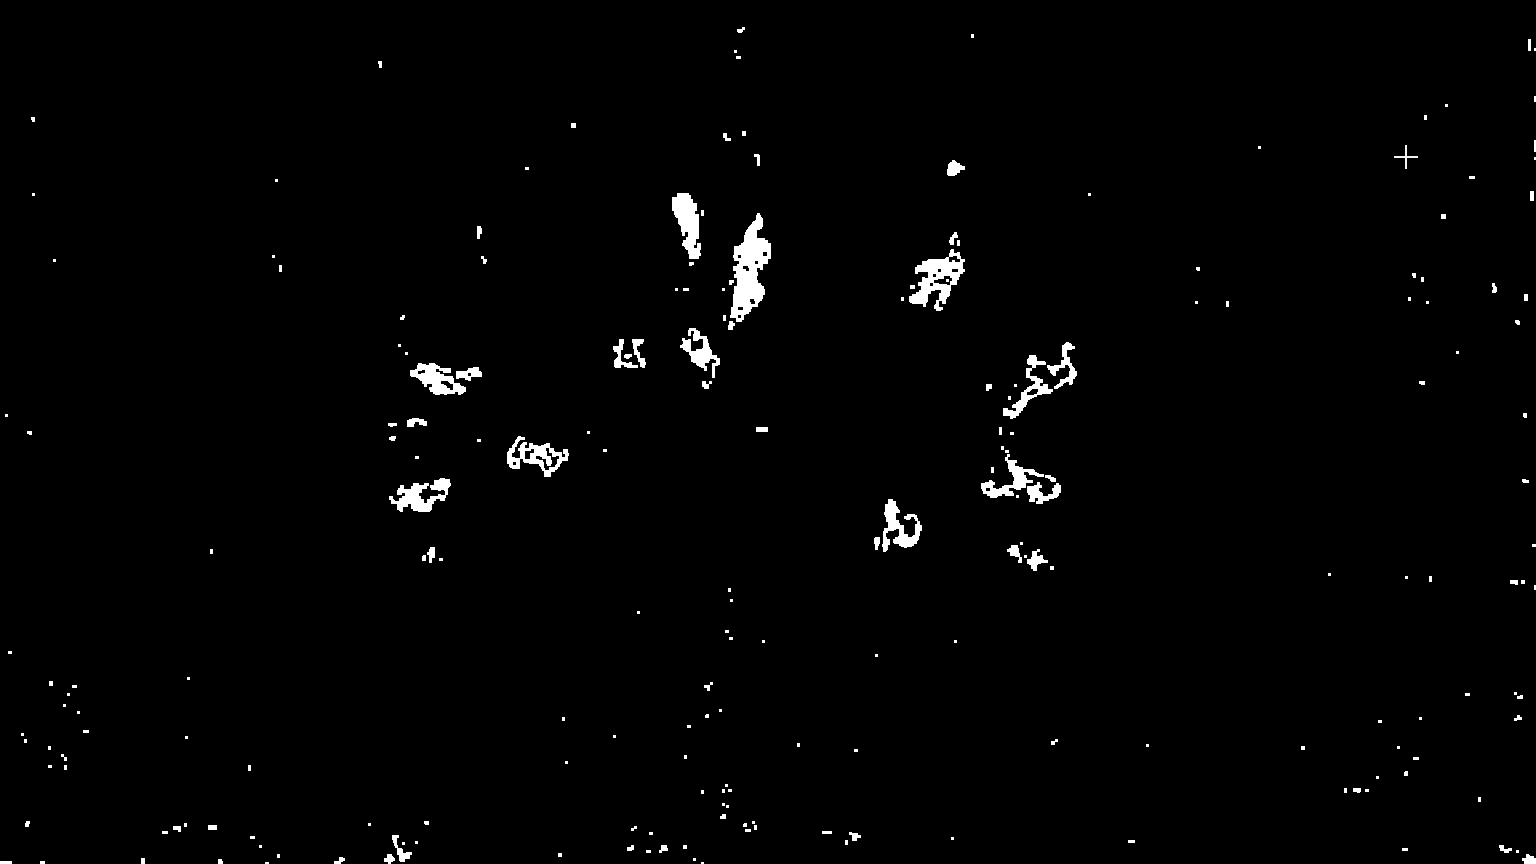
\includegraphics[width=.9\linewidth]{images/CNTsub}
  \caption { }
  \label{fig:CNT1a}
\end{subfigure}%
\begin{subfigure}{.5\textwidth}
  \centering
  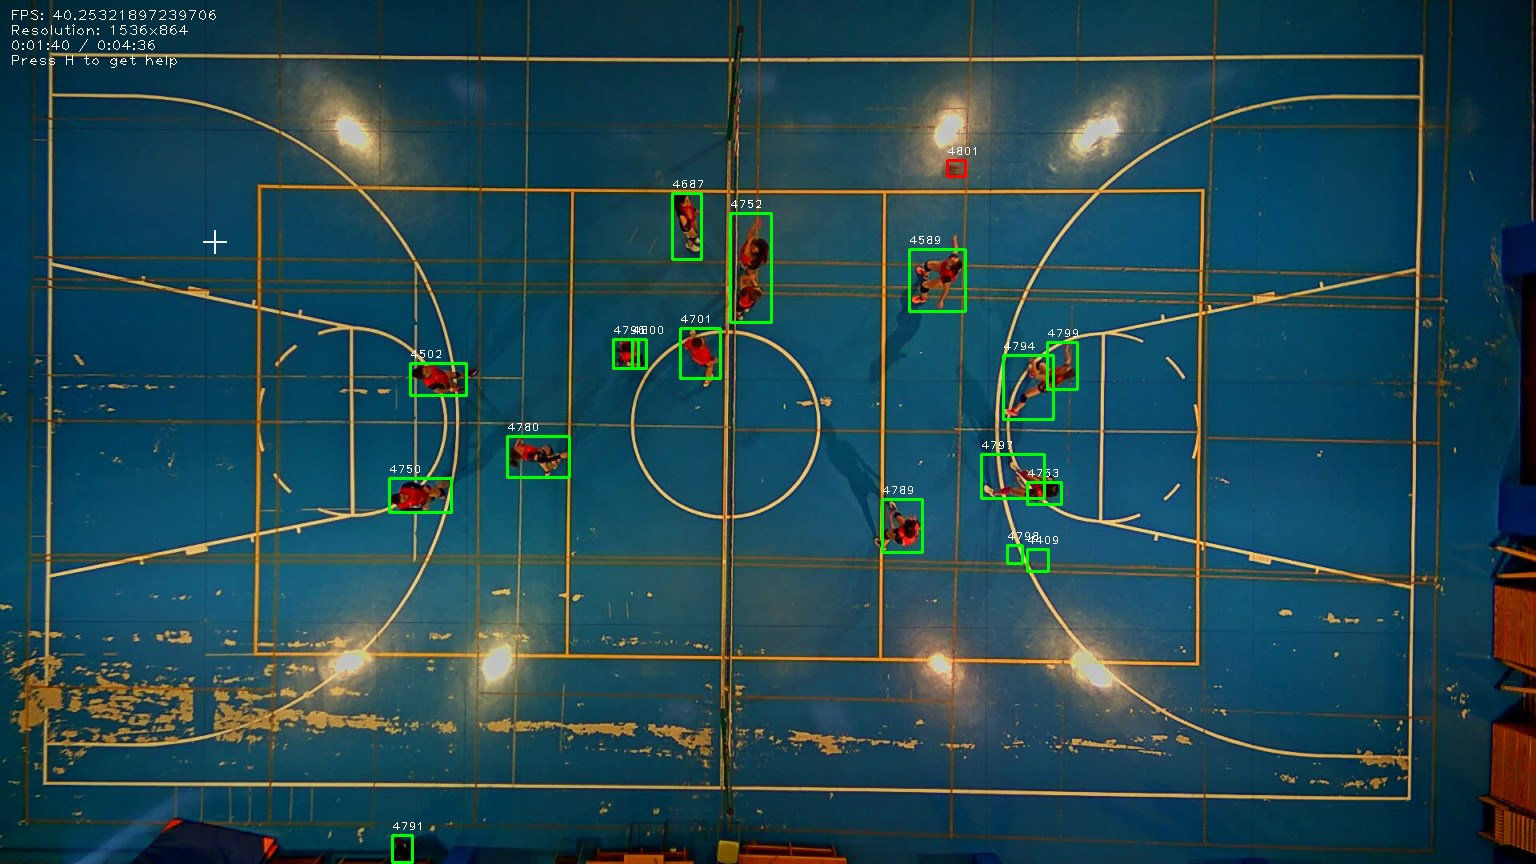
\includegraphics[width=.9\linewidth]{images/CNT}
  \caption { }
  \label{fig:CNT1b}
\end{subfigure}
\caption{Salida del algoritmo CNT (a) Imagen binarizada del algoritmo (b) Imagen del vídeo tras aplicar la máscara }
\label{fig:CNT}
\end{figure}

En mi caso, usando este método, la reproducción del vídeo llega sobradamente a los 30 fps, con lo que puede ser útil si existe la necesidad de que la aplicación funcione en tiempo real, además de contar con un modo para paralelizar la ejecución de manera que sea incluso más rápida. Sin embargo, se aprecian problemas de ruido en la imagen binarizada, lo cual crea varios contornos falsos.

\subsubsection*{GSOC}
GSOC fue implementado durante un \textit{Google Summer of Code}, no procede de ningún artículo, sino que parte de un algoritmo existente (LSBP). El funcionamiento de este algoritmo no tiene documentación más allá de aclarar que se basa en ¿¿saliencia de vídeo??

En general, el algoritmo funciona de manera bastante robusta en lo que respecta a detectar formas en la escena, e incluso es capaz de detectar sin grandes problemas las sombras. Sin embargo, no logra detectar el balón de manera consistente, por lo que sería necesario usar algún tipo de algoritmo de tracking en conjunción a este.

\begin{figure}
\begin{subfigure}{.5\textwidth}
  \centering
  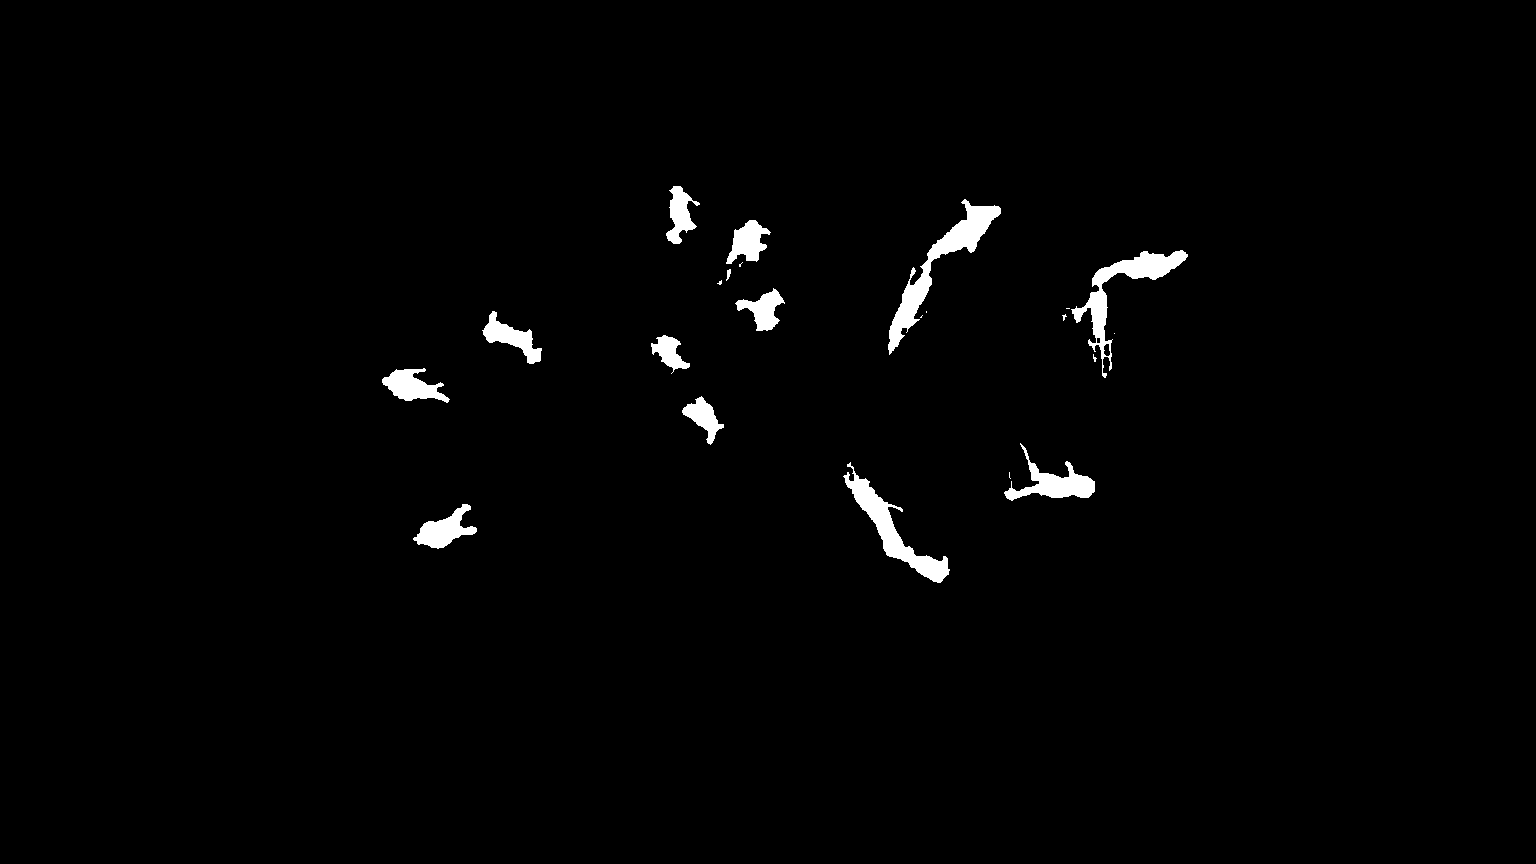
\includegraphics[width=.9\linewidth]{images/GSOCsub}
  \caption { }
  \label{fig:GSOC1a}
\end{subfigure}%
\begin{subfigure}{.5\textwidth}
  \centering
  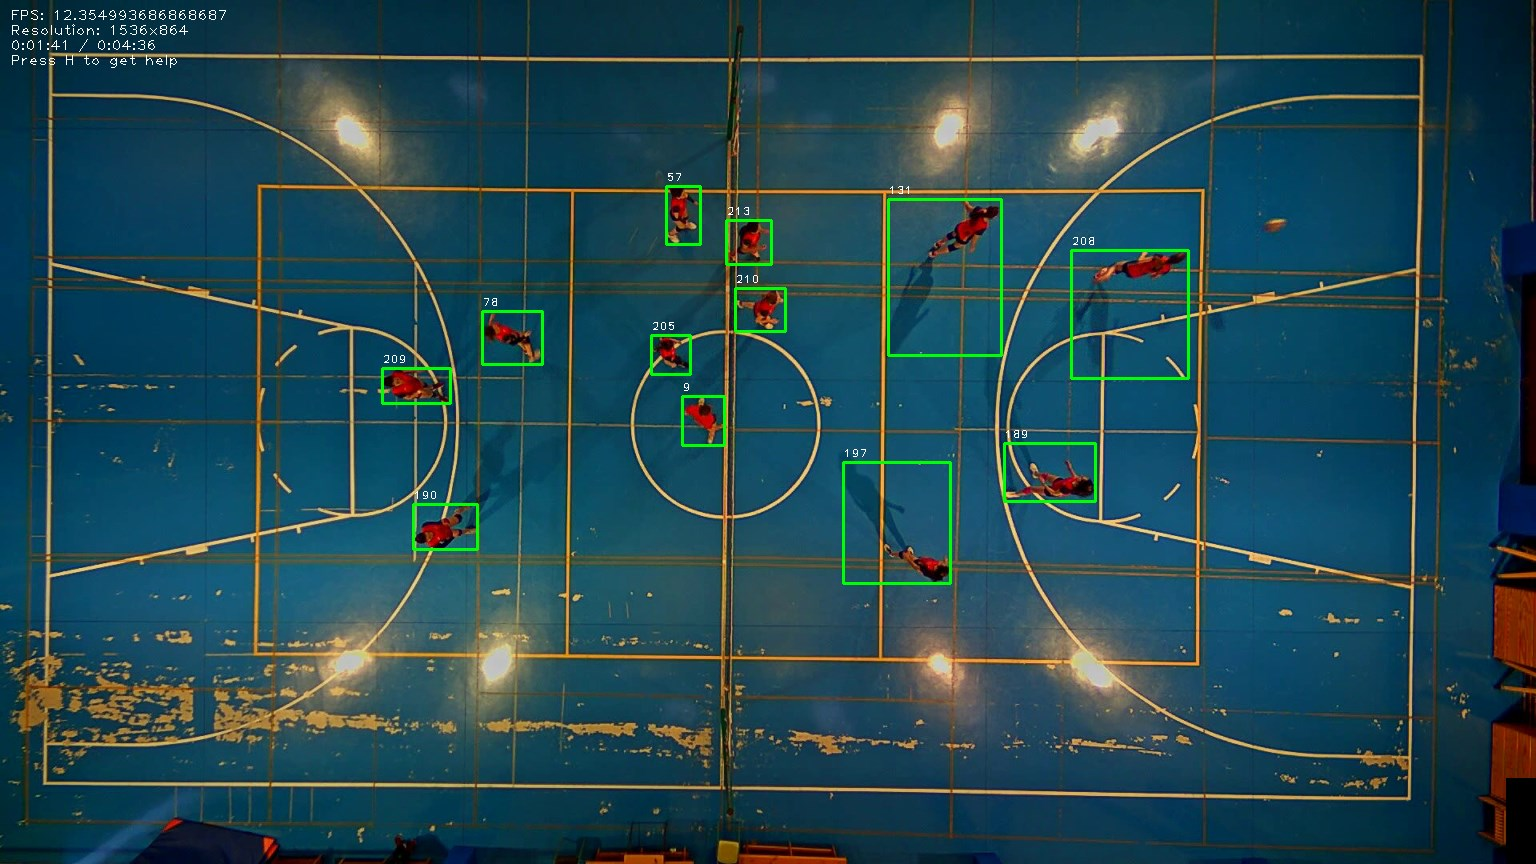
\includegraphics[width=.9\linewidth]{images/GSOC}
  \caption { }
  \label{fig:GSOC1b}
\end{subfigure}
\caption{Salida del algoritmo GSOC (a) Imagen binarizada del algoritmo (b) Imagen del vídeo tras aplicar la máscara }
\label{fig:GSOC}
\end{figure}

Por otro lado, a pesar de su robustez, el algoritmo es el más lento de los que se han probado, lo que lo hace bastante desaconsejable para aplicaciones en tiempo real.

\subsubsection*{KNN}
\begin{figure}[H]
    \centering
    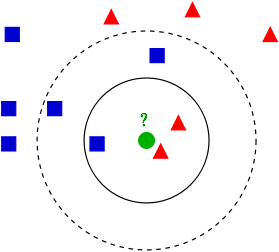
\includegraphics[width=0.3\textwidth]{images/knnejemplo}
    \caption{Ejemplo de funcionamiento de KNN en entorno bidimensional con $k=3$ en línea continua y $k=5$ en línea discontinua}
    \label{fig:knnejemplo}
\end{figure}

KNN \cite{Bishop:2006:PRM:1162264}, también conocido como método de los k-vecinos más cercanos, es un algoritmo bastante popular en reconocimiento de patrones. Es un método de clasificación supervisada no paramétrico.

\begin{figure}
\begin{subfigure}{.5\textwidth}
  \centering
  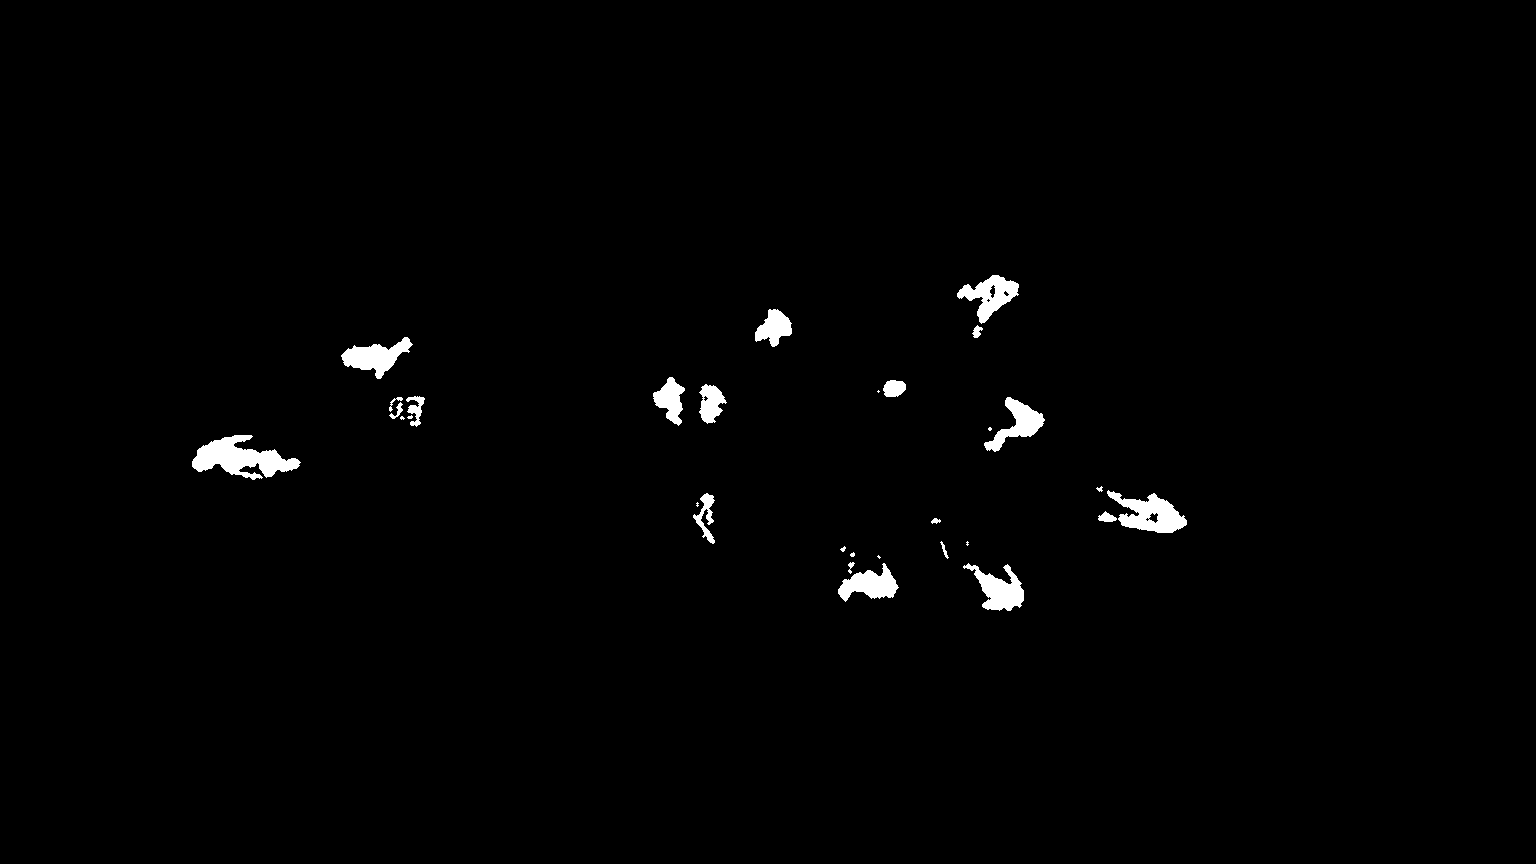
\includegraphics[width=.9\linewidth]{images/KNNsub}
  \caption { }
  \label{fig:KNN1a}
\end{subfigure}%
\begin{subfigure}{.5\textwidth}
  \centering
  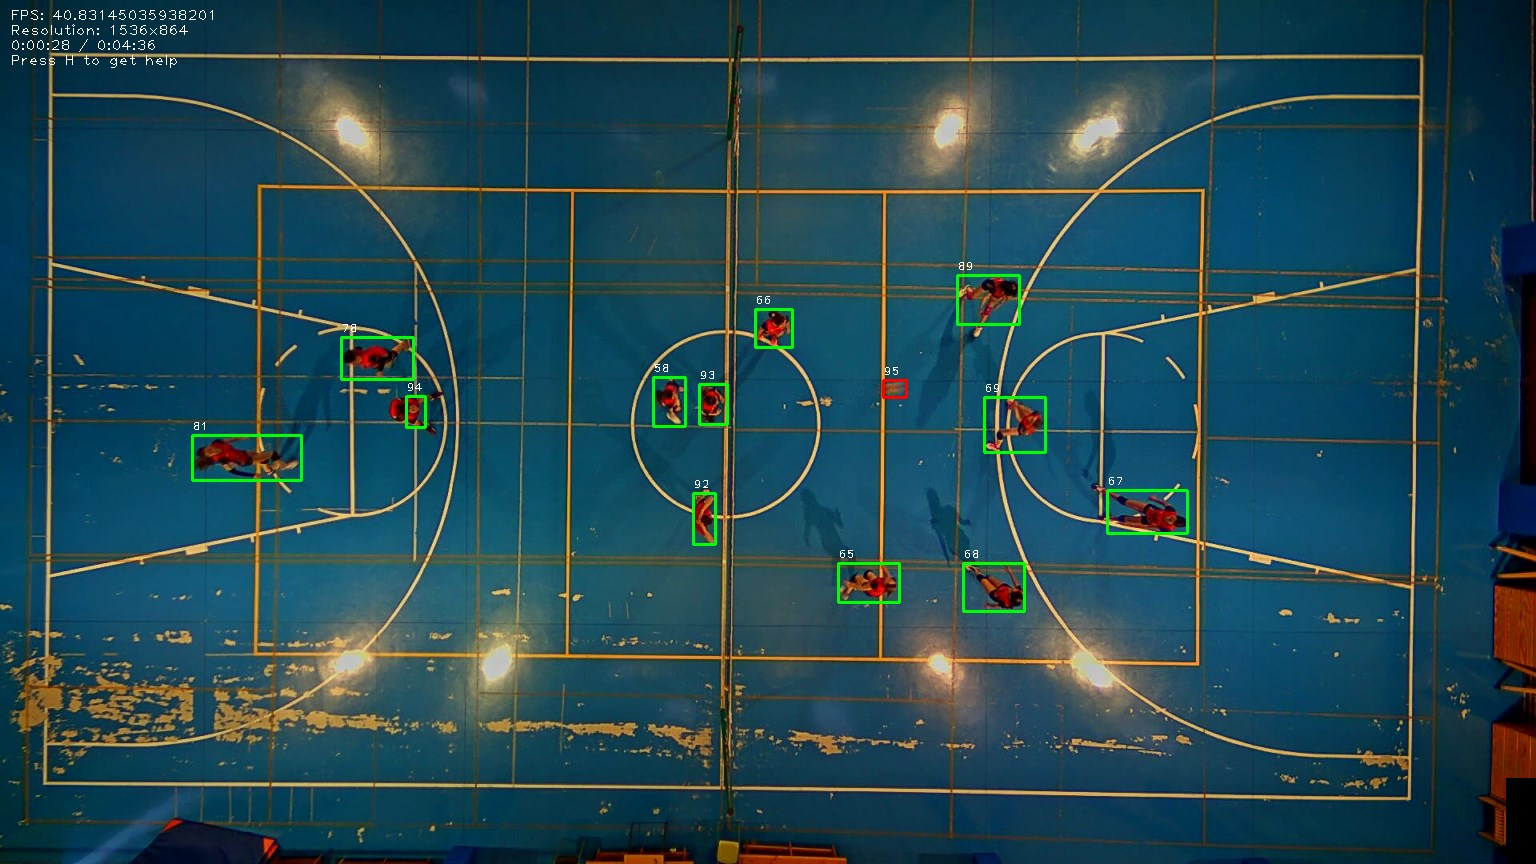
\includegraphics[width=.9\linewidth]{images/KNN}
  \caption { }
  \label{fig:KNN1b}
\end{subfigure}
\caption{Salida del algoritmo KNN (a) Imagen binarizada del algoritmo (b) Imagen del vídeo tras aplicar la máscara }
\label{fig:KNN}
\end{figure}

La base del funcionamiento algoritmo es sencilla: dados unos datos etiquetados, y un punto nuevo del que no conocemos su clase, se trata de inferir a qué clase pertenece calculando las distancias a los k vecinos más cercanos. La clase del punto será la misma que tenga la mayoría de sus k vecinos. Por ejemplo, en la figura \ref{fig:knnejemplo} podemos ver cómo el círculo verde, que es del que desconocemos su clase, tiene, con $k=3$ como vecinos 2 triángulos y 1 cuadrado, por lo que se etiquetaría como triángulo. Si por el contrario tenemos $k=5$, entonces hay 3 cuadrados y 2 triángulos como vecinos más cercanos, en cuyo caso se etiquetaría como cuadrado.

Dado que en el caso de la sustracción de fondo no tenemos datos etiquetados a priori, se debe realizar una primera estimación, por lo tanto, durante un número de frames iniciales $n$, se guardan las $n$ ternas RGB que actuarán como el modelo de fondo inicial. Estos datos se toman como si fueran fondo. A continuación, se calculan las $k$ distancias de cada pixel nuevo a los $T$ anteriores y dependiendo de las distancias, se estima la probabilidad de ser fondo o no. El modelo de fondo se va actualizando, sustituyendo vectores antiguos por vectores nuevos que se consideran fondo.

Según Zivkovic \cite{art:Zivkovic2}, se adapta el tamaño del kernel $k$ a cada pixel. En lugar de buscar un tamaño óptimo global, se incrementa para cada pixel hasta que haya una cantidad suficiente de datos. De esa forma se logran $k$ grandes en áreas con un pequeño número de muestras y $k$ pequeños en zonas con muchas muestras. Es común usar $k=1$, pero se recomienda $k=0.1T$ para mayor robustez a valores atípicos.

\subsubsection*{Operaciones posteriores}

\begin{figure}
\begin{subfigure}{.5\textwidth}
  \centering
  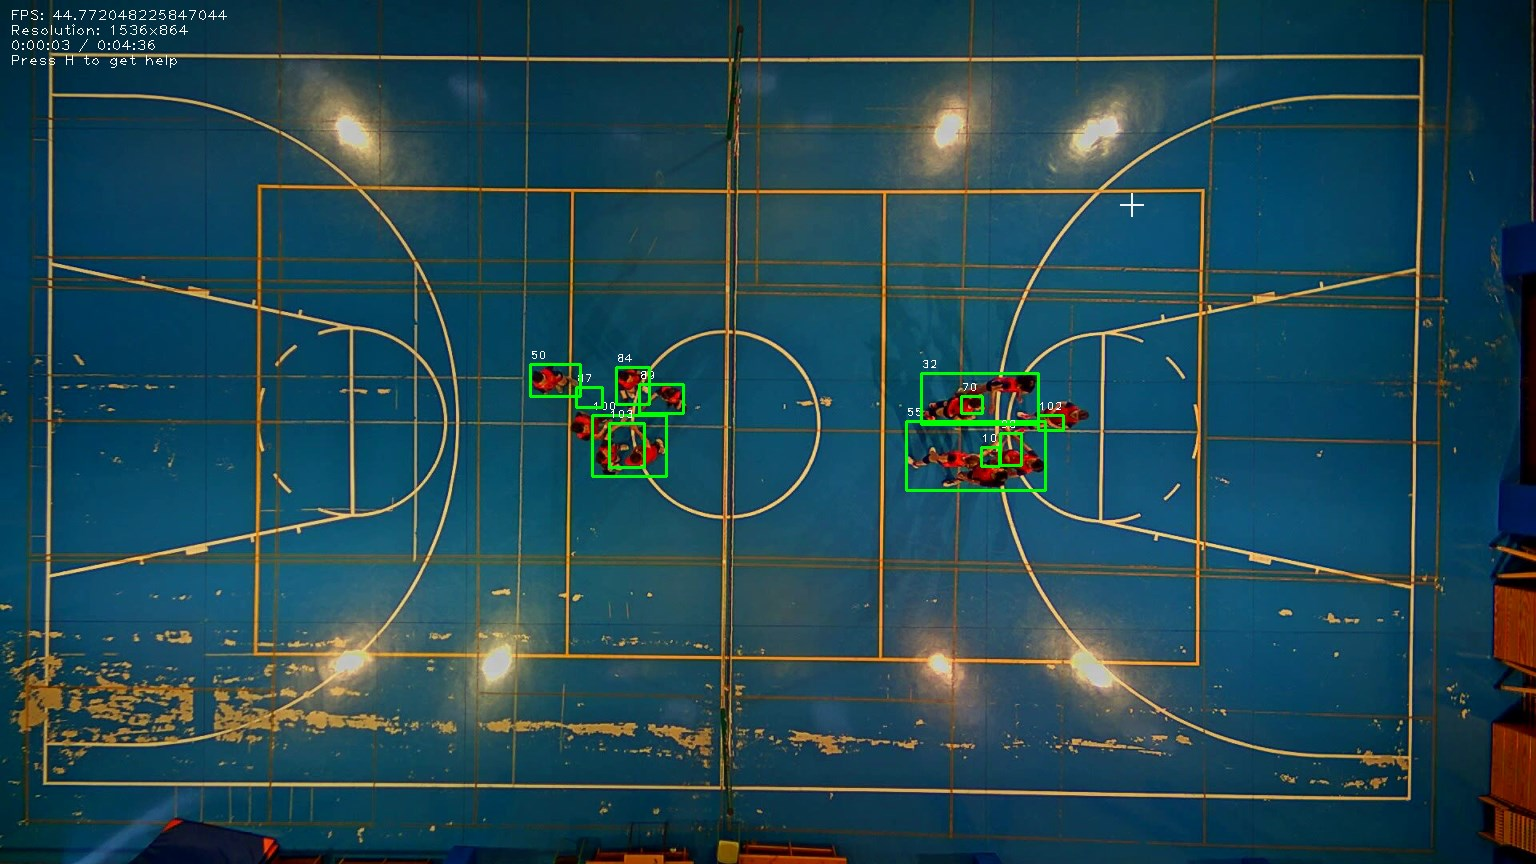
\includegraphics[width=.9\linewidth]{images/nonms}
  \caption { }
  \label{fig:nms1a}
\end{subfigure}%
\begin{subfigure}{.5\textwidth}
  \centering
  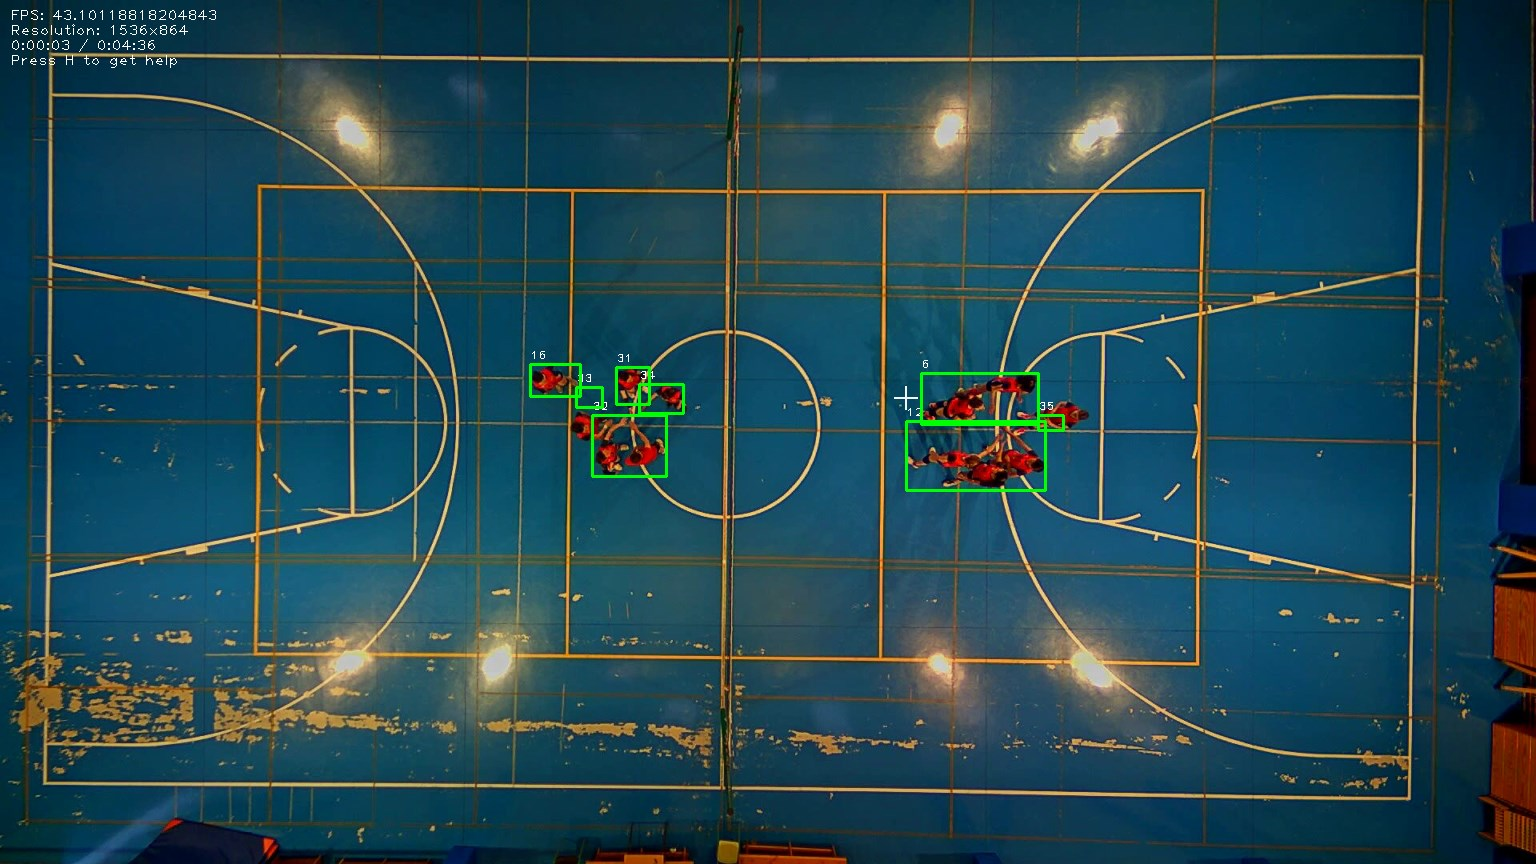
\includegraphics[width=.9\linewidth]{images/nms}
  \caption { }
  \label{fig:nms1b}
\end{subfigure}
\caption{Comparativa de la salida del vídeo antes (a) y después (b) de aplicar la operación de supresión de no máximos }
\label{fig:nms}
\end{figure}

La primera de ellas es la \textbf{supresión de no máximos}. En ciertos momentos del vídeo, puede que no se detecte una forma de manera completa, sino que se detecta el contorno y ciertas partes separadas. Cuando esto ocurre, la imagen de salida tiene la forma que vemos en la figura \ref{fig:nms1a} donde pueden verse varios cuadrados redundantes que podrían englobarse en uno más grande. Tras aplicar la supresión de no máximos, la imagen queda como en la figura \ref{fig:nms1b}, donde puede verse que los cuadrados contenidos dentro de otros han sido suprimidos.

La segunda operación es el \textbf{test de circularidad}, el cual nos sirve para saber cuál de las formas detectadas en la imagen es el balón. Para ello, calculamos el coeficiente de circularidad $C =  \frac{4*\pi*\acute{a}rea}{per\acute{\imath}metro^2}$. Cuanto mayor sea $C$, mayor probabilidad de que la forma sea la de un círculo, es decir, la del balón. En un frame cualquiera, la forma cuyo coeficiente $C$ tenga un valor mayor de 0.6 y sea el mayor de todos los contornos detectados, se marcará en rojo en la imagen de salida, mientras que el resto se marcarán en verde.

La última de las operaciones que se realizan es el etiquetado de los contornos detectados. Esto es importante ya que, de un frame a otro, no tenemos una manera rápida de saber qué contorno del frame actual corresponde con qué contorno del anterior. Para solucionar esta problemática, en el primer frame se da una etiqueta a todos los contornos que se detecta. A partir de aquí, en los siguientes frames se irá etiquetando en base a un emparejamiento mutuo entre los contornos, calculando una matriz de distancias de todos los contornos entre sí. Una vez calculada esta matriz, si para un contorno $c$, su más cercano es otro contorno $k$ y si para $k$ el más cercano es $c$, esto quiere decir que son el mismo contorno. En caso de quedar contornos sin pareja después de esto, simplemente se les da una etiqueta nueva.

\subsubsection*{Comparativa entre algoritmos}

Ahora tendremos que seleccionar de entre todos los algoritmos anteriores el que mejor convenga a nuestros objetivos, teniendo en cuenta el coste computacional de cada uno, así como su desempeño a la hora de estimar el fondo.

El primer apartado a valorar será el rendimiento en frames por segundo (FPS) de cada algoritmo con distintos tamaños de imagen. Cabe aclarar que la cifra de FPS que aparece en la tabla no se mantiene constante sino que es un promedio de las cifras observadas durante la ejecución. Suponiendo que la escala 1 de imagen es la resolución original, 1920x1080, los resultados obtenidos son:

\begin{center}
    \begin{tabular}{| l | c | c | c |}
    \hline
    \textbf{Método} & \textbf{FPS a escala 1} & \textbf{FPS a escala 0.8} & \textbf{FPS a escala 0.6}\\ \hline
    Diferencia de frames & 40 & 51 & 68 \\ \hline
    MOG & 15 & 23 & 37 \\ \hline
    MOG2 & 28 & 36 & 52 \\ \hline
    GMG & 10 & 15 & 24 \\ \hline
    CNT & 30 & 41 & 55\\ \hline
    KNN & 32 & 40 & 56\\ \hline
    
    \end{tabular}
\end{center}

Podemos ver que CNT y KNN son los dos mejores en lo que a velocidad se refiere, con valores de fps muy parejos, seguidos por MOG2. Por otro lado, GMG es de todos los métodos el más lento con diferencia.

Como se ha visto antes, MOG2 es sensiblemente más rápido que MOG debido a que se adapta el número de mezclas por zonas de la imagen, haciendo que el procesamiento de cada frame sea más rápido si se necesitan menos mezclas gaussianas.

Mención aparte merece el método de resta de frames, ya que, aunque es el que mejores números tiene, su detección no es especialmente buena debido a la sensibilidad a cambios de iluminación, por lo que, a pesar de su buena velocidad, seguimos manteniéndolo como descartado.

CNT es también otro descarte a pesar de estar entre los tres más rápidos, debido a su falta de estabilidad y robustez a la hora de detectar formas, que lo hace poco útil en nuestro caso concreto. 

\begin{figure}
\begin{subfigure}{.5\textwidth}
  \centering
  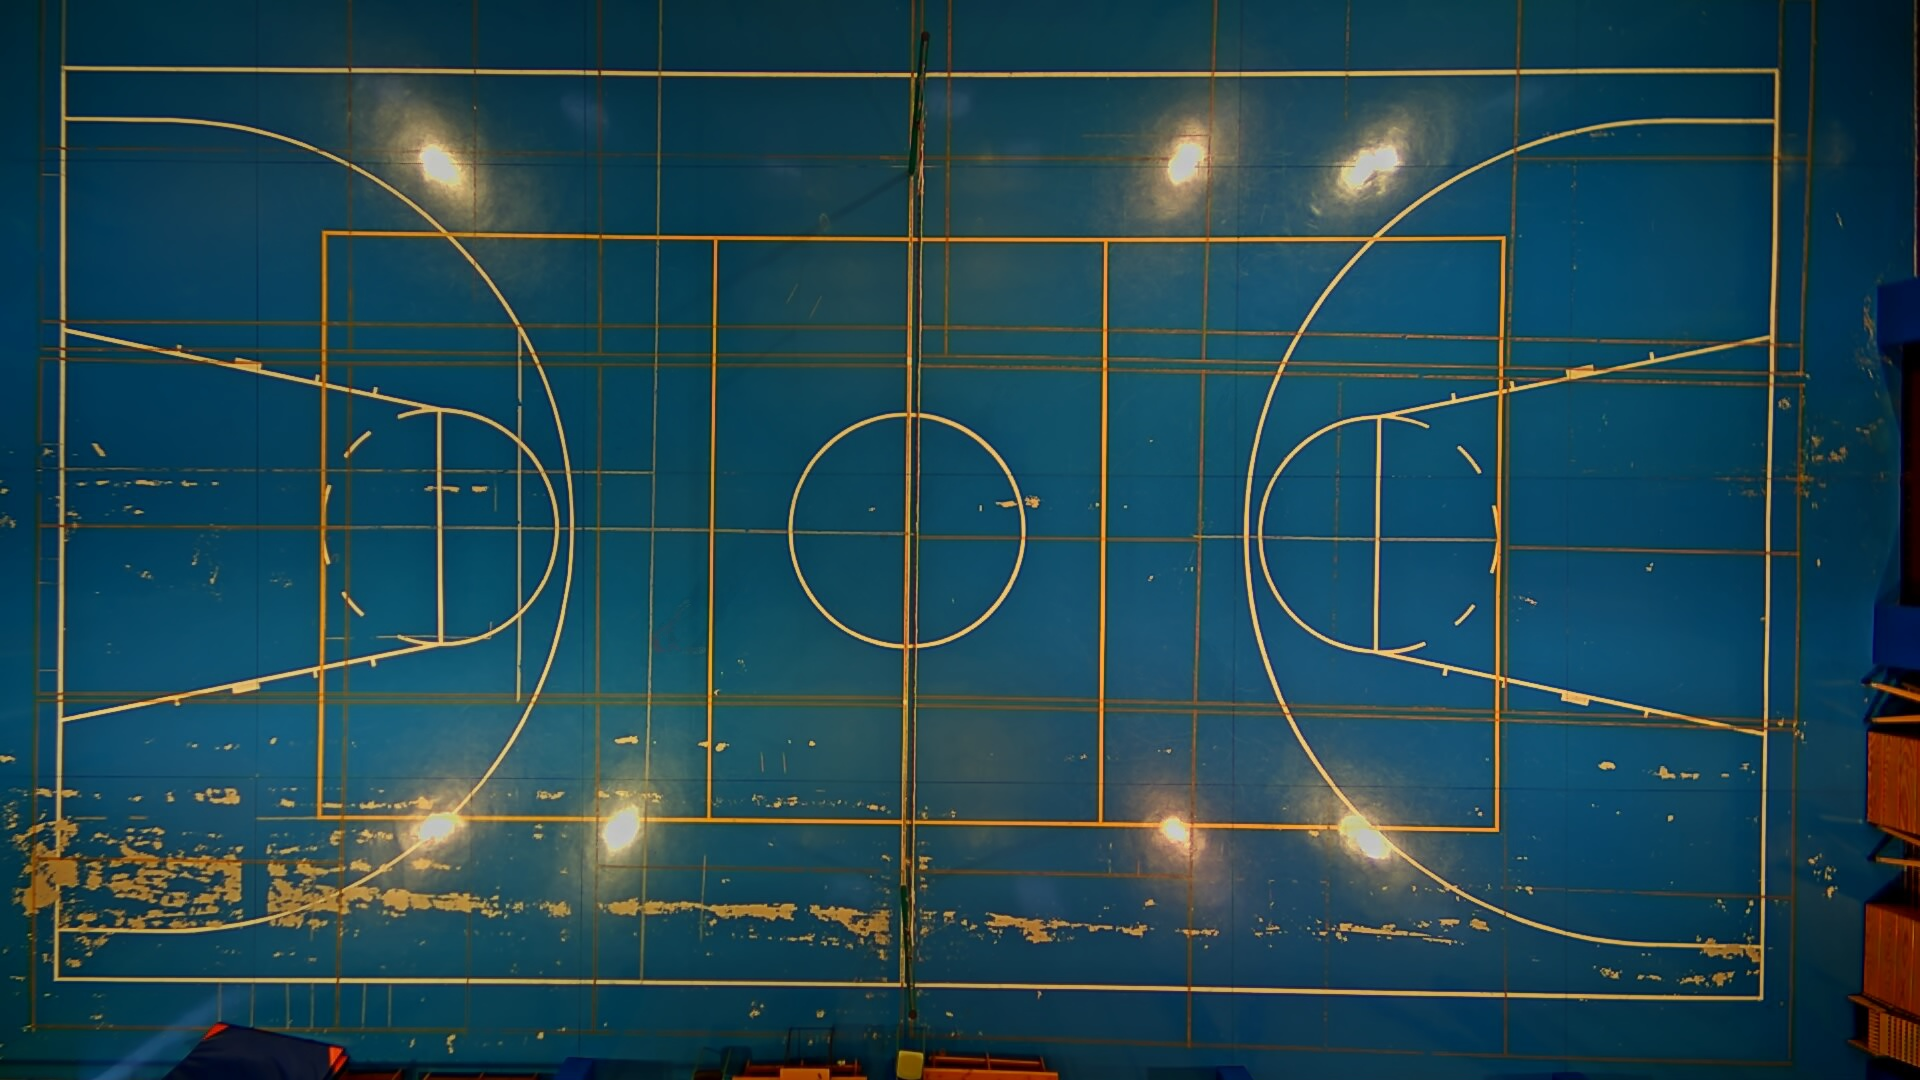
\includegraphics[width=.9\linewidth]{images/modeloMOG}
  \caption { }
  \label{fig:modelos1a}
\end{subfigure}%
\begin{subfigure}{.5\textwidth}
  \centering
  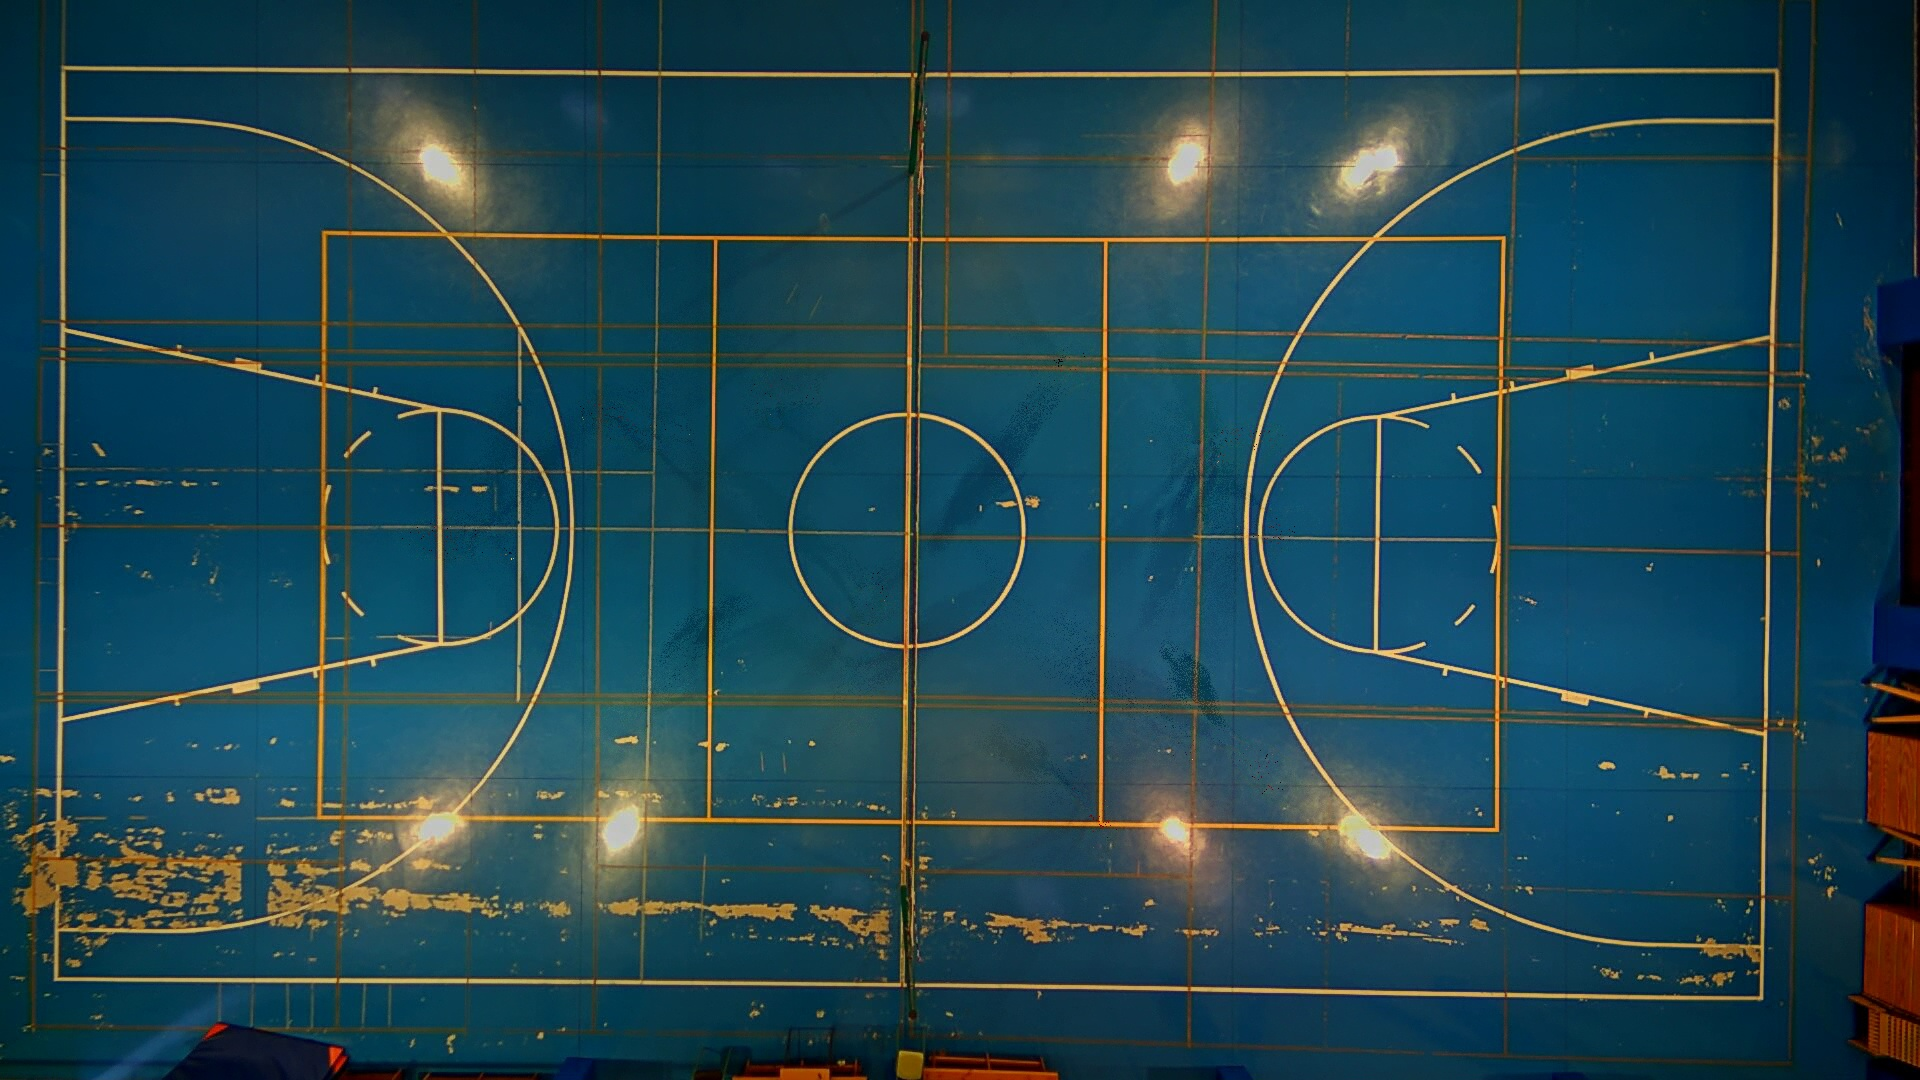
\includegraphics[width=.9\linewidth]{images/modeloKNN}
  \caption { }
  \label{fig:modelos1b}
\end{subfigure}
\caption{Comparativa entre los modelos de fondo finales de MOG2 (a) y KNN (b) tras un vídeo de un set completo }
\label{fig:modelos}
\end{figure}

Con lo cual, nos toca decidir entre MOG2 y KNN, que son los dos candidatos que nos quedan atendiendo a la velocidad de ambos. Ambos tienen una detección muy parecida, pero MOG2 es ligeramente superior a la hora de estimar el modelo de fondo (En la figura \ref{fig:modelos} se puede ver que el modelo de MOG2 es más limpio). También es mejor MOG2 en ciertas ocasiones a la hora de detectar sombras. Por estos motivos, sumados a que la velocidad no es un requisito principal del trabajo, se usará MOG2 como método principal para sustracción de fondo.

\subsection{Seguimiento}
Otra manera mediante la que podemos detectar a las jugadoras y al balón es el seguimiento o \textit{tracking}. Cabe aclarar que no necesariamente es excluyente el uso de esta técnica con el de sustracción de fondo, sino que puede servir para complementar a esta en ciertos objetos que el sustractor de fondo no detecte correctamente.

Nuevamente, OpenCV pone a nuestra disposición una 2 algoritmos de seguimiento: Mean Shift y CAMShift. El módulo colaborativo añade otros cuantos más. Al igual que en el apartado anterior, se usará la programación orientada a objetos para crear una jerarquía de clases que haga sencilla la selección del algoritmo a usar, proporcionando una interfaz común al programar.

Los algoritmos de seguimiento que proporciona el módulo colaborativo de OpenCV son Boosting, MIL, Median Flow y TLD, y fueron los primeros que se probaron e implementaron. Los resultados no fueron muy satisfactorios con ninguno de ellos, tanto en velocidad como en detección de los algoritmos.

\begin{figure}
    \centering
    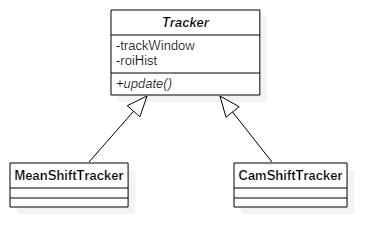
\includegraphics[width=0.35\textwidth]{images/trackers}
    \caption{Estructura de clases de los algoritmos de \textit{tracking}}
    \label{fig:trackers}
\end{figure}

Tras descartar los anteriores métodos, se implementaron los métodos de Mean Shift y CAMShift. Como se ha dicho antes, se ha utilizado una estructura de clases parecida a la de los sustractores de fondo (figura \ref{fig:trackers}) con el mismo objetivo: dar una interfaz común a todas las clases que haga sencillo el seleccionar el algoritmo que se quiera utilizar antes de ejecutar el programa.

\subsubsection*{Mean Shift}
Mean Shift es una técnica de análisis de espacios de características no paramétrica que consiste en localizar los máximos de una función de densidad, es decir, es un algoritmo de búsqueda de modas. Fue presentada por Fukunaga y Hostetler en 1975 \cite{1055330}. Entre sus aplicaciones se encuentran procesamiento y segmentación de imágenes y, por supuesto, seguimiento o \textit{tracking}.

\begin{figure}
    \centering
    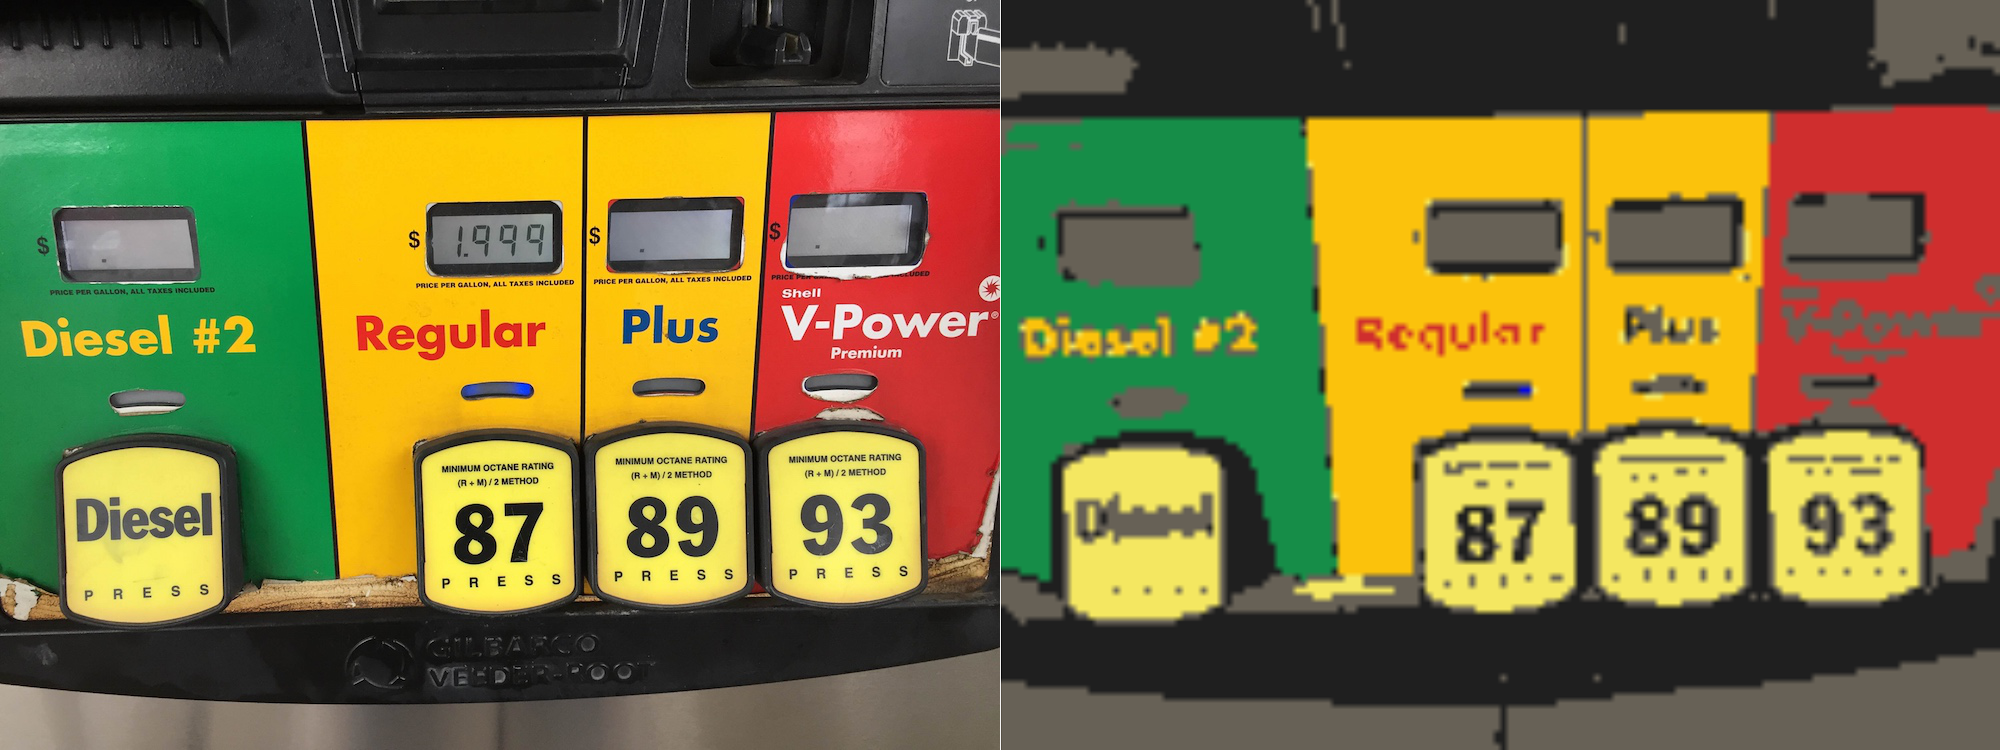
\includegraphics[width=0.6\textwidth]{images/clustering}
    \caption{Ejemplo de aplicación de Mean Shift para clustering}
    \label{fig:clustering}
\end{figure}

El algoritmo de Mean Shift, como se ha dicho, tiene como objetivo la búsqueda de máximos de una función de densidad dada. Para hacerlo, se calcula de manera iterativa a partir de una estimación $x$, conocida como ventana. Una vez proporcionada una ventana al algoritmo, se calculan los pesos de todos los puntos de alrededor de $x$ mediante una función $K$, que normalmente suele tener la forma $K(x_i-x) = e^{-e||x_i-x||^2}$. La media pesada de la densidad en la ventana es:
\[
  m(x) = \frac{\sum_{x_i\in N(x)}K(x_i-x)x_i}{\sum_{x_i\in N(x)}K(x_i-x)}
\]
siendo $N(x)$ el conjunto de vecinos en $x$.

La diferencia $m(x)-x$ es lo que se llama \textit{mean shift} (literalmente: desplazamiento de media) en el trabajo de Fukunaga y Hostetler. En la siguiente iteración se hace $x= m(x)$ y se repite hasta que $m(x)$ converge al mismo valor, con un cierto margen de error. En la figura \ref{fig:pasosmshift} se ve un ejemplo de aplicación de algoritmo, los puntos del conjunto de datos original en azul y los modificados por Mean Shift en rojo. Puede verse claramente que los puntos rojos acaban convergiendo a sus modas locales.

Ahora bien, en el caso del seguimiento, el algoritmo varía levemente. La ventana inicial es una región de interés de la imagen, a la cual se le calcula el histograma. En cada frame del vídeo, se calcula la retroproyección, es decir, la probabilidad de que un pixel de la imagen pertenezca a la distribución que describe el histograma inicial. Una vez calculado esto, se calcula, iterativamente, el centro de masas de los puntos localizados dentro de la ventana. Como se ha dicho antes, el algoritmo converge cuando el centroide calculado coincide con el centro de la ventana con un cierto margen de error.

\begin{figure}
    \centering
    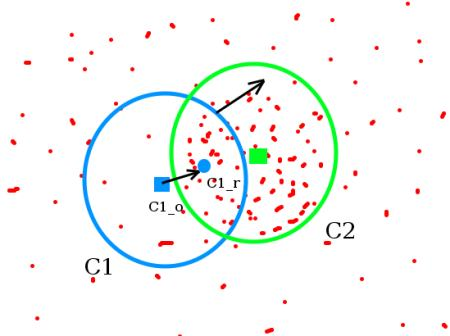
\includegraphics[width=0.4\textwidth]{images/meanshiftopencv}
    \caption{Diagrama de funcionamiento de Mean Shift aplicado a tracking}
    \label{fig:meanshiftopencv}
\end{figure}


Entre las ventajas de Mean Shift se encuentra si capacidad para manejar y adaptarse a distintos espacios de características, además de, en el caso de la segmentación, que no es necesario dar un número de clusters de datos, sino que el algoritmo es capaz de hallarlos por sí mismo. Sin embargo, es un algoritmo más bien lento (tiene un orden de $n^2$) aunque fácilmente paralelizable, y, en el caso del seguimiento, dado que el tamaño de la ventana es constante, puede tener problemas en caso de que algún objeto de la escena cambie de tamaño (se acerque o bien se aleje, como en la figura \ref{fig:ejemplos1a})

\begin{figure}
  \centering
  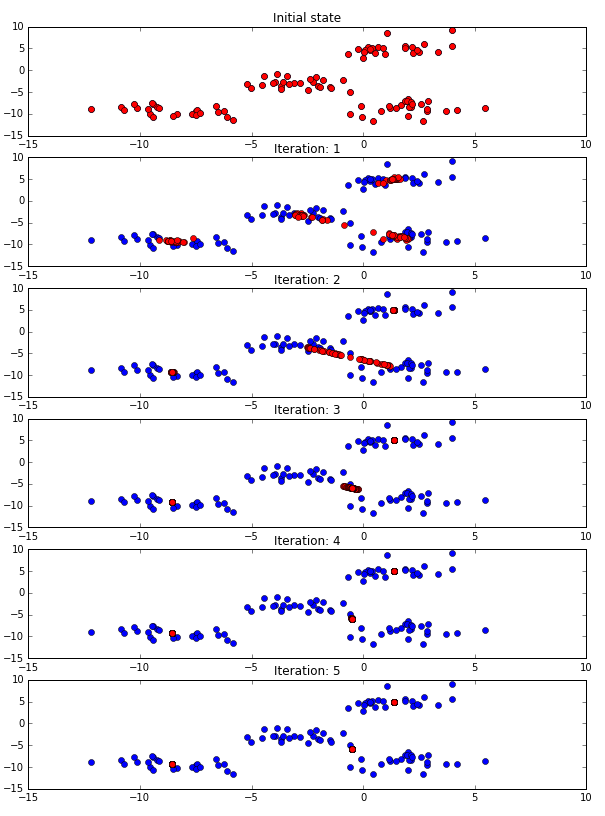
\includegraphics[width=0.4\textwidth]{images/pasosmshift}
  \caption{Mean Shift aplicado a una nube de puntos iteración a iteración}
  \label{fig:pasosmshift}
\end{figure}

\subsubsection*{CAMShift}

CAMShift es una versión adaptativa del algoritmo anterior propuesta por Gary Bradski \textit{et al.} \cite{art:camshift}. Básicamente, este método soluciona la falta de adaptabilidad de la ventana de Mean Shift. Para ello, se aplica en cada frame Mean Shift de la misma manera que se ha expuesto en el apartado anterior. La diferencia es que en este caso, tras la aplicación de Mean Shift, se calculan $M_{00}$, $M_{20}$ y $M_{02}$, definidos por:
\[
  M_{00} = \sum_x \sum_y I(x,y) ; M_{20} = \sum_x \sum_y x^2 I(x,y) ; M_{02} = \sum_x \sum_y y^2 I(x,y)
\]

Siendo $I(x,y)$ la probabilidad en la posición $(x,y)$. Con estos valores se calculan los parámetros de la nueva ventana: orientación $\theta$, longitud $l$ y anchura $w$. Sea

\[
a = \frac{M_{20}}{M_{00}} - x_c^2 ; b = 2(\frac{M_{11}}{M_00}-x_cy_c) ; c = \frac{M_{02}}{M_{00}} - y_c^2
\]
La nueva ventana puede calcularse como
\begin{gather*}
  \theta = \frac{\arctan \frac{2b}{a-c}}{2} \\
  l = \sqrt{\frac{(a+c)+\sqrt{b^2+(a-c)^2}}{2}} \\
  w = \sqrt{\frac{(a+c)-\sqrt{b^2+(a-c)^2}}{2}}
\end{gather*}

El resto del método es exactamente igual que Mean Shift, se hace uso de un histograma y retroproyecciones para calcular el centro de la ventana. Por ello, el resultado obtenido es igualmente bueno con la ventaja de que se adapta a cambios de tamaño en los objetos de la escena. Sin embargo, CAMShift es ligeramente más costoso de procesar, debido a los cálculos necesarios para hallar las medidas de la ventana.

\subsubsection*{Comparativa y selección}

\begin{figure}
  \begin{subfigure}{.5\textwidth}
    \centering
    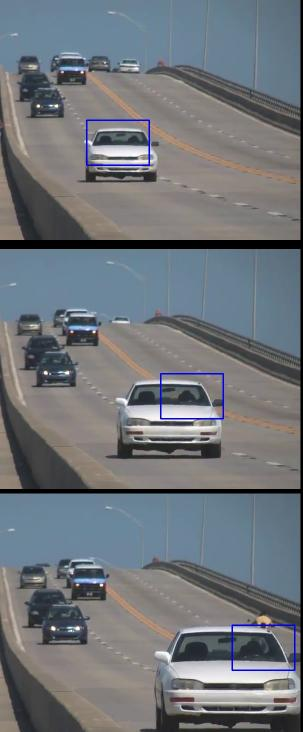
\includegraphics[width=.45\textwidth]{images/cochemeanshift}
    \caption{}
    \label{fig:ejemplos1a}
  \end{subfigure}
  \begin{subfigure}{.4\textwidth}
    \centering
    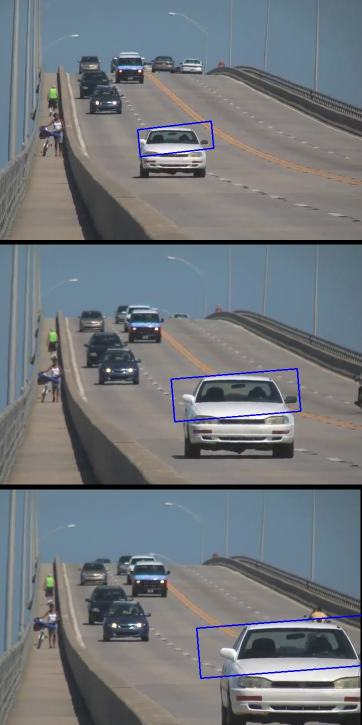
\includegraphics[width=0.65\textwidth]{images/cochecamshift}
    \caption{ }
    \label{fig:ejemplos1b}
  \end{subfigure}
  \caption{Ejemplos de tracking usando Mean Shift y CAMShift (a) Usando Mean Shift (b) Usando CAMShift}
  \label{fig:ejemplos}
\end{figure}

En la mayoría de entornos, la adaptabilidad de CAMShift lo hace superior en lo que a seguimiento se refiere. Sin embargo, esta mejora tiene un pequeño coste computacional. 


En el caso que nos ocupa, dado que la cámara es fija, los objetos no se alejan ni acercan a ella, con la salvedad del balón, que aun con todo, vuelve a alejarse rápidamente y no resulta un problema para su seguimiento. Debido a esto, y para evitar un coste computacional adicional que no nos resultaría especialmente útil, se ha optado por Mean Shift como algoritmo de seguimiento por defecto.

\subsection{Interfaz gráfica}


